
\documentclass[reqno,11pt]{amsart}

%\usepackage{color,graphicx}
%\usepackage{mathrsfs,amsbsy}
\usepackage{amssymb}
\usepackage{amsmath}
\usepackage{amsfonts}
\usepackage{bm}
\usepackage{caption,subcaption}
\usepackage{graphicx}
\usepackage{amsthm}
\usepackage{enumerate}
\usepackage[mathscr]{eucal}
\usepackage{float}
\usepackage{mathrsfs}
\usepackage{multicol}
\usepackage{multirow}
\usepackage[all,pdf]{xy}
\usepackage[a4paper,left=3cm,right=3cm]{geometry}
\usepackage[table,xcdraw]{xcolor} % before tikz-cd
\usepackage{tikz-cd}
\usepackage{quiver} 
\usepackage{resizegather}
\usepackage{diagbox}
\usepackage{hyperref}
\hypersetup{
colorlinks=true,
linkcolor=blue,
urlcolor=blue,
}
%\usepackage[notcite,notref]{showkeys}

% showkeys  make label explicit on the paper

\makeatletter
\@namedef{subjclassname@2010}{%
  \textup{2010} Mathematics Subject Classification}
\makeatother

\numberwithin{equation}{section}

\theoremstyle{plain}
\newtheorem{theorem}{Theorem}[section]
\newtheorem{lemma}[theorem]{Lemma}
\newtheorem{proposition}[theorem]{Proposition}
\newtheorem{corollary}[theorem]{Corollary}
\newtheorem{claim}[theorem]{Claim}
\newtheorem{conj}[theorem]{Conjecture}
\newtheorem{defn}[theorem]{Definition}
\newtheorem{ques}[theorem]{Question}
\newtheorem*{fact}{Facts}
\newtheorem{eg}[theorem]{Example}
\newtheorem*{notation}{Conventions and Notations}

\theoremstyle{plain}
\newtheorem{thmsub}{Theorem}[subsection]
\newtheorem{lemmasub}[thmsub]{Lemma}
\newtheorem{corollarysub}[thmsub]{Corollary}
\newtheorem{propositionsub}[thmsub]{Proposition}
\newtheorem{defnsub}[thmsub]{Definition}

\numberwithin{equation}{section}


\theoremstyle{remark}

\newtheorem{remark}[theorem]{Remark}
\newtheorem{remarks}{Remarks}

%\renewcommand\thefootnote{\fnsymbol{footnote}}
%dont use number as footnote symbol, use this command to change

\DeclareMathOperator{\supp}{supp}
\DeclareMathOperator{\dist}{dist}
\DeclareMathOperator{\vol}{vol}
\DeclareMathOperator{\diag}{diag}
\DeclareMathOperator{\tr}{tr}
\DeclareMathOperator{\Img}{\operatorname{Im}}
\DeclareMathOperator{\Id}{\operatorname{Id}}
\DeclareMathOperator{\rep}{\operatorname{rep}}
\DeclareMathOperator{\Mod}{\operatorname{mod}}
\DeclareMathOperator{\Hom}{\operatorname{Hom}}
\DeclareMathOperator{\Ext}{\operatorname{Ext}}
\DeclareMathOperator{\Mor}{\operatorname{Mor}}
\DeclareMathOperator{\rad}{\operatorname{rad}}
\DeclareMathOperator{\ind}{\operatorname{ind}}
\DeclareMathOperator{\End}{\operatorname{End}}
\DeclareMathOperator{\Jac}{\operatorname{Jac}}
\DeclareMathOperator{\Spec}{\operatorname{Spec}}
\DeclareMathOperator{\Modup}{\overline{\operatorname{mod}}}
\DeclareMathOperator{\Moddown}{\underline{\operatorname{mod}}}
\DeclareMathOperator{\Homup}{\overline{\operatorname{Hom}}}
\DeclareMathOperator{\Homdown}{\underline{\operatorname{Hom}}}
\DeclareMathOperator{\gldim}{\operatorname{gl.dim}}
\DeclareMathOperator{\projdim}{\operatorname{proj.dim}}
\DeclareMathOperator{\injdim}{\operatorname{inj.dim}}
\DeclareMathOperator{\dimv}{\operatorname{\underline{\mathbf{dim}}}}


\DeclareMathOperator{\Flagd}{\operatorname{Flag}_{d}}
\DeclareMathOperator{\Flagdstr}{\operatorname{Flag}_{d,\operatorname{str}}}
\newcommand{\Gr}{\operatorname{Gr}}
\newcommand{\Grr}{\operatorname{Gr}}
\newcommand{\Gralg}[1]{\operatorname{Gr}^{#1}}
\newcommand{\Grq}{\operatorname{Gr}^{KQ}}
\newcommand{\Flag}[1]{\operatorname{Flag}_{#1}}
\newcommand{\Flagstr}[1]{\operatorname{Flag}_{#1,\operatorname{str}}}
\newcommand{\dimvec}[1]{\boldsymbol{#1}}
\newcommand{\ord}{\operatorname{ord}}
\newcommand{\orde}{\operatorname{ord}_e }
\newcommand{\shorttimes}{\!\times\!}
\newcommand{\oder}{\;\;\text{ or }\;\;}
\newcommand{\representation}[2]{\genfrac{}{}{0pt}{3}{\phantom{000}#2\phantom{00}}{#1}}
%https://tex.stackexchange.com/questions/96549/how-do-i-write-above-a-left-right-arrow
\makeatletter
\newcommand\xleftrightarrow[2][]{%
  \ext@arrow 9999{\longleftrightarrowfill@}{#1}{#2}}
\newcommand\longleftrightarrowfill@{%
  \arrowfill@\leftarrow\relbar\rightarrow}
\makeatother
\setlength\intextsep{0cm}
\setlength\textfloatsep{0cm}

%%%% todo notes %%%%
\usepackage[colorinlistoftodos,textsize=footnotesize]{todonotes}
\setlength{\marginparwidth}{2.5cm}
\newcommand{\leftnote}[1]{\reversemarginpar\marginnote{\footnotesize #1}}
\newcommand{\rightnote}[1]{\normalmarginpar\marginnote{\footnotesize #1}\reversemarginpar}

\begin{document}
\date{}

\title
{Affine paving of quiver partial flag variety}


\author{Xiaoxiang Zhou}
\address{School of Mathematical Sciences\\
University of Bonn\\
Bonn, 53115\\ Germany\\} 
\email{email:xx352229@mail.ustc.edu.cn}





\begin{abstract}
In this article, we construct affine pavings for quiver partial flag varieties when the quiver is of Dynkin type. To achieve our results, we extend methods from Cerulli-Irelli--Esposito--Franzen--Reineke
 and Maksimau as well as techniques from Auslander--Reiten theory.
\end{abstract}



\maketitle
\tableofcontents
%%%%%%%%%%%%%%%%%%%%%%%%%%%%%%%%%%%%%%%%%%%%%%%%%%%%%%%%%%%%%%%%%%%%%%%%%%%%%%%%%%%%%%%%%%%%%
%quiver partial flag varietie
\section{Introduction}
Affine pavings are an important concept in algebraic geometry similar to cellular decompositions in topology. A complex algebraic variety $X$ has an affine paving if $X$ has a filtration
$$0= X_0 \subset X_1 \subset \cdots \subset X_d=X$$
with $X_i$ closed and $X_{i+1} \setminus X_i$ isomorphic to some affine space $\mathbb{A}^k_{\mathbb{C}}$.

Affine pavings imply nice properties about the cohomology of varieties, for example the vanishing of cohomology in odd degrees. For other properties see \cite[1.7]{de1988homology}.

Affine pavings have been constructed in many cases, as for Grassmannians, flag varieties, as well as certain Springer fibers, quiver Grassmannians, and quiver flag varieties. This article focuses on the case of (strict) partial flag varieties which parameterize subrepresentations of a fixed indecomposable representation of a quiver. In particular, we consider quivers of Dynkin type or affine type.
In this case, affine pavings have been constructed in \cite{irelli2019cell} for quiver Grassmannians in all types and in \cite{maksimau2019flag} for partial flag varieties of type $A$ and $D$ (see Table \ref{table:result}). Besides, affine pavings 
have been constructed in \cite[Theorem 6.3]{eberhardt2022motivic} for strict partial flag varieties in type $\tilde{A}$ with cyclic orientation, which generalized the result in \cite{sauter2015cell} for complete quiver flag varieties in nilpotent representations of an oriented cycle. In this paper, we will tackle the remaining cases.


%The nocolor version 
\renewcommand{\arraystretch}{1.3}
\begin{table}[ht]
\vspace{0.5cm}
\begin{tabular}{|c|c|c|c|}
\hline
            & $\Grq(X)$                  & $\Flagd(X)$                          & $\Flagdstr(X)$          \\ \hline
$A$         & \multirow{3}{*}{\cite[Section 5]{irelli2019cell}} & \multirow{2}{*}{\cite[Theorem 2.20]{maksimau2019flag}}        & \multirow{2}{*}{Theorem \ref{thm:Dynkincase}}       \\ \cline{1-1}
$D$         &                            &                                      &                         \\ \cline{1-1} \cline{3-4} 
$E$         &                            & \multicolumn{2}{c|}{Theorem \ref{thm:Dynkincase}}                                          \\ \hline
$\tilde{A}$ & \multirow{3}{*}{\cite[Section 6]{irelli2019cell}} & \multicolumn{2}{c|}{\multirow{2}{*}{Section \ref{sec:affine}}}                         \\ \cline{1-1}
$\tilde{D}$ &                            & \multicolumn{2}{c|}{}                                          \\ \cline{1-1} \cline{3-4} 
$\tilde{E}$ &                            & \multicolumn{2}{c|}{reduced to the regular quasi-finite case.} \\ \hline
\end{tabular}
\vspace{1mm}
\caption{}\label{table:result}
\end{table}

We proceed as follows. In Section \ref{sec:flag=gr}, we discuss basic definitions and properties of partial flags. In Section \ref{sec:mainthm} we will prove key Theorems \ref{thm:main1} and \ref{thm:main2}, which allow us to construct affine pavings for quiver partial flag varieties inductively. We apply these theorems to partial flag varieties of Dynkin type, see Section \ref{sec:Dynkin}, and to partial flag varieties of affine type, see Section \ref{sec:affine}. We will combine and extend results from \cite{irelli2019cell} and \cite{maksimau2019flag}.
Following the arguments of \cite{maksimau2019flag} would require studying millions of cases when we  consider the Dynkin quivers of type $E$. To avoid this, we extend the methods of \cite{irelli2019cell} from quiver Grassmannian to quiver partial flag variety. This will reduce the case by case analysis to a feasible computation of (mostly) 8 critical cases, which we carry out in Section \ref{sec:Dynkin} and Appendix \ref{appendix:proofcomplement}. The reduction uses Auslander--Reiten theory which we recall in Appendix \ref{appendix:arth}.
%It's easy to see that $\Flag{1}(X)=\Grq(X)$. These geometrical objects can be divided into different pieces according to the dimension vectors of $M_1,\ldots,M_d$, and each piece have its own natural (complex/Zariski) topology. It was proved in \cite{irelli2019cell} that $\Grq(X)$ have an affine paving, and in \cite{maksimau2019flag} that $\Flagd(X)$ have the same property when $Q$ is Dynkin quiver of type $A/E$. Here we go one step further, the results are concluded in the Table \ref{table:result}.
%
%
%The idea of proof is very simple: first, we view the  quiver partial flag variety as the quiver Grassmannian of the more complicated quiver; then we establish the decomposition so that one may solve the problem by induction; finally we set a special way of decomposition for each indecomposable module so that we can avoid meeting the bad decomposition. These contents are in Section \ref{sec:flag=gr},\ref{sec:mainthm},\ref{sec:Dynkin}, accordingly.
\begin{notation}
Throughout this article, $K=\mathbb{C}$, $R$ is a $K$-algebra with unit, and $\Mod(R)$ denotes the category of $R$-modules of finite dimension. Let $Q$ be a quiver equipped with the set of finite vertices $v(Q)$ and the set of finite edges $a(Q)$. For an
arrow $b$, we call $s(b)$ the starting vertex and $t(b)$ the terminal vertex
of $b$. We denote by $KQ$ the path algebra and $\rep(Q)=\Mod(KQ)$ the category of quiver representations of finite dimension. For a representation $X\in \rep(Q)$, we denote by $X_i:=e_iX$ the $K$-linear space at the vertex $i\in v(Q)$. We denote by $P(i)$, $I(i)$ and $S(i)$ the indecomposable projective, injective, simple modules corresponding to the vertex $i$, respectively.
\end{notation}


%%%%%%%%%%%%%%%%%%%%%%%%%%%%%%%%%%%%%%%%%%%%%%%%%%%%%%%%%%%%%%%%%%%%%%%%%%%%%%%%%%%%%%%%%%%%%
\section*{Acknowledgement}
%\addcontentsline{toc}{section}{Acknowledgement}
First, I would like to thank my supervisor, Jens Niklas Eberhardt, for introducing me this specific problem, discussing earlier drafts, as well as providing help with the write-up. I would also like to thank Hans Franzen for answering some questions regarding \cite{irelli2019cell}, and thank Ruslan Maksimau for some comments and suggestions. This article is part of my master thesis project.
%My thanks go to Professor xyz for his / her guidance and advice in the preparation and finalization of this article
% I would like to express my gratitude to
%my advisor James Newton without whom this paper would never have been completed. I
%thank him for suggesting this problem and guiding me throughout the whole project. He
%spent many hours discussing earlier drafts with me and explained a lot of things to me.
\section{Preliminaries}\label{sec:flag=gr}
\subsection{Extended quiver}
In this subsection, we introduce the notion of extended quiver which allows to view partial flag varieties as quiver Grassmannians. Intuitively, a flag of quiver representations can be encoded as a subspace of a representation of the extended quiver.

\begin{defn}[Extended quiver]
For a quiver $Q$ and an integer $d \geqslant 1$, the extended quiver $Q_{d}$ is defined as follows:
\begin{itemize}
	\item The vertex set of $Q_d$ is defined as the Cartesian product of the vertex set of $Q$ and $\{1,\ldots,d\}$, i.e.,
	$$v(Q_d)=v(Q) \times \{1,\ldots,d\}.$$
	\item  There are two types of arrows: for each $(i,r) \in v(Q) \times \{1,\ldots,d-1\}$, there is one arrow from $(i,r)$ to $(i,r+1)$; for each arrow $i \longrightarrow j$ in $Q$ and $r \in \{1,\ldots,d\}$, there is one arrow from $(i,r)$ to $(j,r)$.
\end{itemize}
\end{defn}

The extended quiver $Q_d$ is exactly the same quiver as $\hat{\Gamma}_d$ in \cite[Definition 2.2]{maksimau2019flag}. The next definition is a small variation:

\begin{defn}[Strict extended quiver]
For a quiver $Q$ and an integer $d \geqslant 2$, the strict extended quiver $Q_{d,\operatorname{str}}$ is defined as follows:
\begin{itemize}
	\item The vertex set of $Q_d$ is defined as the Cartesian product of the vertex set of $Q$ and $\{1,\ldots,d\}$, i.e.,
	$$v(Q_{d,\operatorname{str}})=v(Q) \times \{1,\ldots,d\}.$$
	\item  We have two types of arrows: for each $(i,r) \in v(Q) \times \{1,\ldots,d-1\}$, there is one arrow from $(i,r)$ to $(i,r+1)$; for each arrow $i \longrightarrow j$ in quiver $Q$ and $r \in \{2,\ldots,d\}$, there is one arrow from $(i,r)$ to $(j,r-1)$.
\end{itemize}
\end{defn}


\begin{eg}\label{eg:ext_quiver}
The (strict) extended quiver for a Dynkin quiver $Q$ of type $A_4$ looks as follows.
% https://q.uiver.app/?q=WzAsMzEsWzAsMiwiXFxidWxsZXQiXSxbMiwyLCJcXGJ1bGxldCJdLFs0LDIsIlxcYnVsbGV0Il0sWzYsMiwiXFxidWxsZXQiXSxbNywyLCJcXGJ1bGxldCJdLFs5LDIsIlxcYnVsbGV0Il0sWzExLDIsIlxcYnVsbGV0Il0sWzEzLDIsIlxcYnVsbGV0Il0sWzcsMSwiXFxidWxsZXQiXSxbOSwxLCJcXGJ1bGxldCJdLFsxMSwxLCJcXGJ1bGxldCJdLFsxMywxLCJcXGJ1bGxldCJdLFs3LDAsIlxcYnVsbGV0Il0sWzksMCwiXFxidWxsZXQiXSxbMTEsMCwiXFxidWxsZXQiXSxbMTMsMCwiXFxidWxsZXQiXSxbMTQsMiwiXFxidWxsZXQiXSxbMTYsMiwiXFxidWxsZXQiXSxbMTQsMSwiXFxidWxsZXQiXSxbMTQsMCwiXFxidWxsZXQiXSxbMTYsMSwiXFxidWxsZXQiXSxbMTgsMSwiXFxidWxsZXQiXSxbMTgsMCwiXFxidWxsZXQiXSxbMjAsMSwiXFxidWxsZXQiXSxbMjAsMiwiXFxidWxsZXQiXSxbMjAsMCwiXFxidWxsZXQiXSxbMTgsMiwiXFxidWxsZXQiXSxbMTYsMCwiXFxidWxsZXQiXSxbMywzLCJcXGhzcGFjZXstMWNtfVFcXGhzcGFjZXstMWNtfSJdLFsxMCwzLCJcXGhzcGFjZXstMWNtfVFfM1xcaHNwYWNley0xY219Il0sWzE3LDMsIlxcaHNwYWNley0xY219UV97MyxzdHJ9XFxoc3BhY2V7LTFjbX0iXSxbMCwxXSxbMiwxXSxbMiwzXSxbNCw1XSxbNiw1XSxbNiw3XSxbOCw5XSxbMTAsOV0sWzEwLDExXSxbMTIsMTNdLFsxNCwxM10sWzE0LDE1XSxbOCwxMl0sWzQsOF0sWzUsOV0sWzksMTNdLFsxMCwxNF0sWzYsMTBdLFs3LDExXSxbMTEsMTVdLFsxOCwxN10sWzE5LDIwXSxbMjEsMTddLFsyMiwyMF0sWzIyLDIzXSxbMjEsMjRdLFsyMywyNV0sWzI0LDIzXSxbMjYsMjFdLFsyMSwyMl0sWzE3LDIwXSxbMjAsMjddLFsxOCwxOV0sWzE2LDE4XV0=
\[\begin{tikzcd}[column sep=3mm, row sep=5mm]
	&&&&&&&[5mm] \bullet && \bullet && \bullet && \bullet &[5mm] \bullet && \bullet && \bullet && \bullet \\
	&&&&&&& \bullet && \bullet && \bullet && \bullet & \bullet && \bullet && \bullet && \bullet \\
	\bullet && \bullet && \bullet && \bullet & \bullet && \bullet && \bullet && \bullet & \bullet && \bullet && \bullet && \bullet \\[-5mm]
	&&& {\hspace{-1cm}Q\hspace{-1cm}} &&&&&&& {\hspace{-1cm}Q_3\hspace{-1cm}} &&&&&&& {\hspace{-1cm}Q_{3,\operatorname{str}}\hspace{-1cm}}
	\arrow[from=3-1, to=3-3]
	\arrow[from=3-5, to=3-3]
	\arrow[from=3-5, to=3-7]
	\arrow[from=3-8, to=3-10]
	\arrow[from=3-12, to=3-10]
	\arrow[from=3-12, to=3-14]
	\arrow[from=2-8, to=2-10]
	\arrow[from=2-12, to=2-10]
	\arrow[from=2-12, to=2-14]
	\arrow[from=1-8, to=1-10]
	\arrow[from=1-12, to=1-10]
	\arrow[from=1-12, to=1-14]
	\arrow[from=2-8, to=1-8]
	\arrow[from=3-8, to=2-8]
	\arrow[from=3-10, to=2-10]
	\arrow[from=2-10, to=1-10]
	\arrow[from=2-12, to=1-12]
	\arrow[from=3-12, to=2-12]
	\arrow[from=3-14, to=2-14]
	\arrow[from=2-14, to=1-14]
	\arrow[from=2-15, to=3-17]
	\arrow[from=1-15, to=2-17]
	\arrow[from=2-19, to=3-17]
	\arrow[from=1-19, to=2-17]
	\arrow[from=1-19, to=2-21]
	\arrow[from=2-19, to=3-21]
	\arrow[from=2-21, to=1-21]
	\arrow[from=3-21, to=2-21]
	\arrow[from=3-19, to=2-19]
	\arrow[from=2-19, to=1-19]
	\arrow[from=3-17, to=2-17]
	\arrow[from=2-17, to=1-17]
	\arrow[from=2-15, to=1-15]
	\arrow[from=3-15, to=2-15]
\end{tikzcd}\]
\end{eg}

Next, we define the quiver algebras for later use.
\begin{defn}[Algebra of an extended quiver]\label{def:bqa}
For an extended quiver $Q_d$, let $KQ_d$ be the corresponding path algebra, and $I$ be the ideal of $KQ_d$ identifying all the paths with the same sources and targets. The algebra of the extended quiver $Q_d$ is defined as
$$R_d:= KQ_d/I.$$
Similarly, we define the algebra $R_{d,\operatorname{str}}:= KQ_{d,\operatorname{str}}/I$ for the strict extended quiver.
\end{defn}
By abuse of notation, we often abbreviate $R_d$ and $R_{d,\operatorname{str}}$ by $R$. 
\subsection{Canonical functor $\Phi$}
We follow \cite[2.3]{maksimau2019flag} in this subsection with a few variations. 
\begin{defn}[Partial flag]\label{def:pf}
For a quiver representation $X \in \rep(Q)$, a partial flag of $X$ is defined as an increasing sequence of subrepresentation of $X$. For an integer $d \geqslant 1$, we denote
$$\Flagd(X):=\left\{ 0 \subseteq M_1 \subseteq \cdots M_d \subseteq X \right\}$$
as the collection of all partial flags of length $d$, and call it the partial flag variety. 
\end{defn}
\begin{defn}[Strict partial flag]\label{def:spf}
For a quiver representation $X \in \rep(Q)$, a strict partial flag of $X$ is defined as an increasing sequence of subrepresentation $(M_k)_k$ of $X$ such that for any arrow $x \in v(Q)$ and any $k$, we have $x.M_{k+1} \subseteq M_{k}$. For an integer $d \geqslant 2$, we denote
$$\Flagdstr(X):=\left\{ 0 \subseteq M_1 \subseteq \cdots M_d \subseteq X\mid x.M_{k+1} \subseteq M_k \right\}$$
as the collection of all strict partial flags of length $d$, and call it the strict partial flag variety. 
\end{defn}
\begin{defn}[Grassmannian]
Let $R$ be the bounded quiver algebra defined in Definition \ref{def:pf} or \ref{def:spf}. For a module $T \in \Mod(R)$, the Grassmannian $\Gralg{R}(T)$ is defined as the set of all submodules of $T$, i.e.,
$$\Gralg{R}(T):=\{T' \subseteq T \text{ as the submodule}  \}.$$
\end{defn}
\begin{defn}[Canonical functor $\Phi$]
The canonical functor $\Phi:\rep(Q) \longrightarrow \Mod(R) $ is defined as follows:
\begin{itemize}
\item $\left(\Phi(X)\right)_{(i,r)}:=X_i$;
\item $\left(\Phi(X)\right)_{(i,r) \rightarrow (i,r+1)}:=\Id_{X_i}$;
\item Either $\left(\Phi(X)\right)_{(i,r) \rightarrow (j,r)}:=X_{i \rightarrow j}$ for $R=R_d$, \\or $\left(\Phi(X)\right)_{(i,r) \rightarrow (j,r-1)}:=X_{i \rightarrow j}$ for $R=R_{d,\operatorname{str}}$.
\end{itemize}
\end{defn}
The functor $\Phi$ helps to realize a partial flag as a quiver subrepresentation. 
\begin{proposition}\label{prop:flag=gr}
For a representation $X\in \rep(Q)$, the canonical functor $\Phi$ induces isomorphisms
$$\Flagd(X)\cong \Gralg{R_d}(\Phi(X)) \qquad \Flagdstr(X)\cong \Gralg{R_{d,\operatorname{str}}}(\Phi(X)).$$
\end{proposition}
\begin{proof}
The isomorphism maps a flag $M:M_1 \subseteq \cdots \subseteq M_d$ to a representation $\Phi'(M)$ with $\Phi'(M)_{(i,r)}=M_{i,r}$ and obvious morphisms for arrows. The non-strict case is mentioned in \cite[page 4]{maksimau2019flag} and the strict case works similarly.
\end{proof}
%https://tex.stackexchange.com/questions/495252/i-want-to-get-a-big-subset
\begin{eg}\label{eg:bigpic}
Consider the quiver $Q\colon x \longrightarrow y \longleftarrow z \longrightarrow w$, and let $X\colon X_x \longrightarrow X_y \longleftarrow X_z \longrightarrow X_w$ be a representation. The varieties $\Flag{3}(X),\Flagstr{3}(X)$ then arise as quiver Grassmannian as shown in Figure \ref{fig:flagasgr}.
\begin{center}
	\begin{figure}[ht]
		\vspace{0cm}
		\centering
		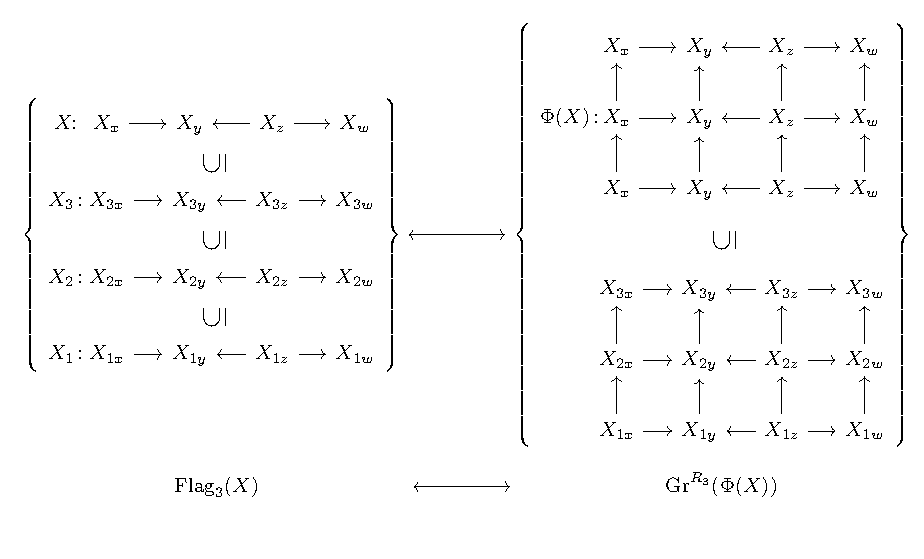
\includegraphics[width=0.9\linewidth]{figures/bigpic.pdf}
		\vspace{-0.5cm}
		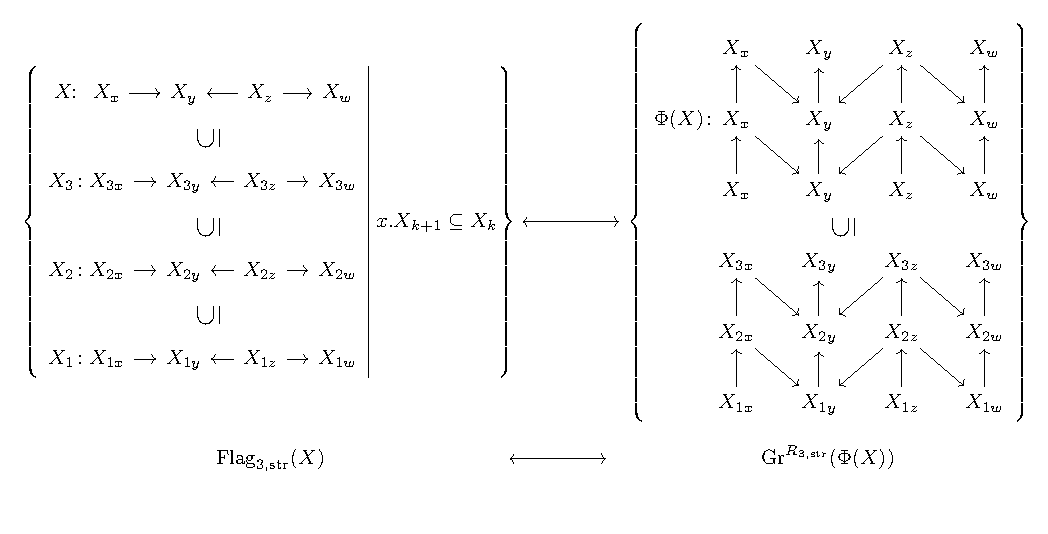
\includegraphics[width=\linewidth]{figures/bigpic2.pdf}
		\vspace{-1cm}
%		\captionsetup{labelformat=empty}
		\caption{}
		\vspace{0.3cm}
		\label{fig:flagasgr}
	\end{figure}
\end{center}
\end{eg}
In many cases, the proof of the strict case and the non-strict case is the same, so we often treat them in the same way. For example, we may abbreviate the formula in Proposition \ref{prop:flag=gr} as 
$$\Flag{}(X)\cong \Gr(\Phi(X)).$$
\subsection{Dimension vector}In this subsection we recall some notations of dimension vectors.
\begin{defn}[Dimension vector]
For a quiver $Q$ and a representation $M \in \rep(Q)$, the set of dimension vectors of $Q$ is defined as $\prod_{i \in v(Q)} \mathbb{Z}$, and the dimension vector of $M$ is defined as
$$\dimv M:=(\dim_K M_i)_{i \in v(Q)}.$$
\end{defn}
Moreover, if $R=KQ/I$ is a bounded quiver algebra, then every module $T \in \Mod(R)$ can be viewed as a representation of $Q$, so we automatically have a notion of dimension vector for $R$ and $T$.

Now we can write the (strict) partial flag variety and Grassmannian as disjoint union of several pieces. Since $v(Q_{d,(\operatorname{str})})=v(Q) \times \{1,\ldots,d\}$, any dimension vector $\dimvec{f}$ of $R$ can be viewed as $d$ dimension vectors $(\dimvec{f_1},\ldots,\dimvec{f_d})$. Define
\begin{equation*}
\begin{aligned}
  \Flagd_{,\dimvec{f}}(X):=\;&\left\{ 0 \subseteq M_1 \subseteq \cdots M_d \subseteq X \;\middle|\; \dimv M_k=\dimvec{f_k} \right\} && \subseteq  \Flagd(X), \\ 
  \Flag{d,\dimvec{f}}^{\operatorname{str}}(X):=\;&\left\{ 0 \subseteq M_1 \subseteq \cdots M_d \subseteq X \;\middle|\; x.M_{k+1} \subseteq M_k,\, \dimv M_k=\dimvec{f_k} \right\} && \subseteq  \Flagdstr(X), \\ 
  \Gralg{R}_{\dimvec{f}}(T):=\;&\{T' \subseteq T \text{ with } \dimv T'=\dimvec{f}\} && \subseteq  \Gralg{R}(T). 
\end{aligned}
\end{equation*}
Then from the Proposition \ref{prop:flag=gr} we get 
$$\Flagd_{,\dimvec{f}}(X) \cong \Gralg{R_d}_{\dimvec{f}}(\Phi(X)) \qquad \Flag{d,\dimvec{f}}^{\operatorname{str}}(X) \cong \Gralg{R_{d,\operatorname{str}}}_{\dimvec{f}}(\Phi(X)).$$
\begin{remark}
All the spaces we defined here have natural topologies and variety structures. For example, by the standard embedding
\[\begin{tikzcd}
	\Gralg{R}_{\dimvec{f}}(T) & \displaystyle\prod_{(i,r) \in v\left(Q_{d,(str)}\right)} \Gr_{\dimvec{f}_{i,r}}\big(T_{(i,r)}\big),
	\arrow[hook, from=1-1, to=1-2]
\end{tikzcd}\]
$\Gralg{R}_{\dimvec{f}}(T)$ is then endowed with the subspace topology and subvariety structure.
\end{remark}


Finally, we need to define the Euler form of two dimension vectors. For this we need to define the set of virtual arrows of the quivers $Q_d$ and $Q_{d,\operatorname{str}}$. Following Example \ref{example:virtualarrow}, the virtual arrows of the quivers $Q_3$ and $Q_{3,\operatorname{str}}$ are depicted in red.
\begin{defn}[Virtual arrows of the quiver $Q_d$]
For $d \geqslant 1$, the virtual arrows of the quiver $Q_d$ is defined as a triple $\big(va(Q_d),s,t\big)$, where
$$va(Q_d):=a(Q) \times \{1,\ldots, d-1 \}$$
is a finite set, and $s,t: va(Q_d) \longrightarrow v(Q_d)$ are maps defined by
$$s\big((i\rightarrow j,r)\big)=(i,r) \qquad t \big((i\rightarrow j,r)\big)=(j,r+1).$$
\end{defn}
\begin{defn}[Virtual arrows of the quiver $Q_{d,\operatorname{str}}$]
For $d \geqslant 2$, the virtual arrows of the quiver $Q_{d,\operatorname{str}}$ is defined as a triple $\big(va(Q_{d,\operatorname{str}}),s,t\big)$, where
$$va(Q_{d,\operatorname{str}}):=a(Q) \times \{2,\ldots, d-1 \}$$
is a finite set, and $s,t: va(Q_{d,\operatorname{str}}) \longrightarrow v(Q_{d,\operatorname{str}})$ are maps defined by
$$s\big((i\rightarrow j,r)\big)=(i,r) \qquad t \big((i\rightarrow j,r)\big)=(j,r).$$
\end{defn}
\begin{eg}\label{example:virtualarrow}
$\qquad$
	\begin{figure}[ht]
		\vspace{0cm}
		\centering
% https://q.uiver.app/?q=WzAsMzEsWzAsMiwiXFxidWxsZXQiXSxbMiwyLCJcXGJ1bGxldCJdLFs0LDIsIlxcYnVsbGV0Il0sWzYsMiwiXFxidWxsZXQiXSxbNywyLCJcXGJ1bGxldCJdLFs5LDIsIlxcYnVsbGV0Il0sWzExLDIsIlxcYnVsbGV0Il0sWzEzLDIsIlxcYnVsbGV0Il0sWzcsMSwiXFxidWxsZXQiXSxbOSwxLCJcXGJ1bGxldCJdLFsxMSwxLCJcXGJ1bGxldCJdLFsxMywxLCJcXGJ1bGxldCJdLFs3LDAsIlxcYnVsbGV0Il0sWzksMCwiXFxidWxsZXQiXSxbMTEsMCwiXFxidWxsZXQiXSxbMTMsMCwiXFxidWxsZXQiXSxbMTQsMiwiXFxidWxsZXQiXSxbMTYsMiwiXFxidWxsZXQiXSxbMTQsMSwiXFxidWxsZXQiXSxbMTQsMCwiXFxidWxsZXQiXSxbMTYsMSwiXFxidWxsZXQiXSxbMTgsMSwiXFxidWxsZXQiXSxbMTgsMCwiXFxidWxsZXQiXSxbMjAsMSwiXFxidWxsZXQiXSxbMjAsMiwiXFxidWxsZXQiXSxbMjAsMCwiXFxidWxsZXQiXSxbMTgsMiwiXFxidWxsZXQiXSxbMTYsMCwiXFxidWxsZXQiXSxbMywzLCJcXGhzcGFjZXstMWNtfVFcXGhzcGFjZXstMWNtfSJdLFsxMCwzLCJcXGhzcGFjZXstMWNtfVFfM1xcaHNwYWNley0xY219Il0sWzE3LDMsIlxcaHNwYWNley0xY219UV97MyxzdHJ9XFxoc3BhY2V7LTFjbX0iXSxbMCwxXSxbMiwxXSxbMiwzXSxbNCw1XSxbNiw1XSxbNiw3XSxbOCw5XSxbMTAsOV0sWzEwLDExXSxbMTIsMTNdLFsxNCwxM10sWzE0LDE1XSxbOCwxMl0sWzQsOF0sWzUsOV0sWzksMTNdLFsxMCwxNF0sWzYsMTBdLFs3LDExXSxbMTEsMTVdLFsxOCwxN10sWzE5LDIwXSxbMjEsMTddLFsyMiwyMF0sWzIyLDIzXSxbMjEsMjRdLFsyMywyNV0sWzI0LDIzXSxbMjYsMjFdLFsyMSwyMl0sWzE3LDIwXSxbMjAsMjddLFsxOCwxOV0sWzE2LDE4XSxbOCwxMywiIiwxLHsiY29sb3VyIjpbMCwxMDAsNjBdfV0sWzQsOSwiIiwxLHsiY29sb3VyIjpbMCwxMDAsNjBdfV0sWzEwLDEzLCIiLDEseyJjb2xvdXIiOlswLDEwMCw2MF19XSxbNiw5LCIiLDEseyJjb2xvdXIiOlswLDEwMCw2MF19XSxbNiwxMSwiIiwxLHsiY29sb3VyIjpbMCwxMDAsNjBdfV0sWzEwLDE1LCIiLDEseyJjb2xvdXIiOlswLDEwMCw2MF19XSxbMTgsMjAsIiIsMSx7ImNvbG91ciI6WzAsMTAwLDYwXX1dLFsyMSwyMCwiIiwxLHsiY29sb3VyIjpbMCwxMDAsNjBdfV0sWzIxLDIzLCIiLDEseyJjb2xvdXIiOlswLDEwMCw2MF19XV0=
\[\begin{tikzcd}[column sep=3mm, row sep=5mm]
	&&&&&&&[5mm] \bullet && \bullet && \bullet && \bullet &[5mm] \bullet && \bullet && \bullet && \bullet \\
	&&&&&&& \bullet && \bullet && \bullet && \bullet & \bullet && \bullet && \bullet && \bullet \\
	\bullet && \bullet && \bullet && \bullet & \bullet && \bullet && \bullet && \bullet & \bullet && \bullet && \bullet && \bullet \\[-5mm]
	&&& {\hspace{-1cm}Q\hspace{-1cm}} &&&&&&& {\hspace{-1cm}Q_3\hspace{-1cm}} &&&&&&& {\hspace{-1cm}Q_{3,\operatorname{str}}\hspace{-1cm}}
	\arrow[from=3-1, to=3-3]
	\arrow[from=3-5, to=3-3]
	\arrow[from=3-5, to=3-7]
	\arrow[from=3-8, to=3-10]
	\arrow[from=3-12, to=3-10]
	\arrow[from=3-12, to=3-14]
	\arrow[from=2-8, to=2-10]
	\arrow[from=2-12, to=2-10]
	\arrow[from=2-12, to=2-14]
	\arrow[from=1-8, to=1-10]
	\arrow[from=1-12, to=1-10]
	\arrow[from=1-12, to=1-14]
	\arrow[from=2-8, to=1-8]
	\arrow[from=3-8, to=2-8]
	\arrow[from=3-10, to=2-10]
	\arrow[from=2-10, to=1-10]
	\arrow[from=2-12, to=1-12]
	\arrow[from=3-12, to=2-12]
	\arrow[from=3-14, to=2-14]
	\arrow[from=2-14, to=1-14]
	\arrow[from=2-15, to=3-17]
	\arrow[from=1-15, to=2-17]
	\arrow[from=2-19, to=3-17]
	\arrow[from=1-19, to=2-17]
	\arrow[from=1-19, to=2-21]
	\arrow[from=2-19, to=3-21]
	\arrow[from=2-21, to=1-21]
	\arrow[from=3-21, to=2-21]
	\arrow[from=3-19, to=2-19]
	\arrow[from=2-19, to=1-19]
	\arrow[from=3-17, to=2-17]
	\arrow[from=2-17, to=1-17]
	\arrow[from=2-15, to=1-15]
	\arrow[from=3-15, to=2-15]
	\arrow[color={rgb,255:red,255;green,51;blue,51}, from=2-8, to=1-10]
	\arrow[color={rgb,255:red,255;green,51;blue,51}, from=3-8, to=2-10]
	\arrow[color={rgb,255:red,255;green,51;blue,51}, from=2-12, to=1-10]
	\arrow[color={rgb,255:red,255;green,51;blue,51}, from=3-12, to=2-10]
	\arrow[color={rgb,255:red,255;green,51;blue,51}, from=3-12, to=2-14]
	\arrow[color={rgb,255:red,255;green,51;blue,51}, from=2-12, to=1-14]
	\arrow[color={rgb,255:red,255;green,51;blue,51}, from=2-15, to=2-17]
	\arrow[color={rgb,255:red,255;green,51;blue,51}, from=2-19, to=2-17]
	\arrow[color={rgb,255:red,255;green,51;blue,51}, from=2-19, to=2-21]
\end{tikzcd}\]
\vspace{-5mm}
		\label{fig:virtualarrow}
		\vspace{2mm}
	\end{figure}
\end{eg}
\begin{defn}[Euler form of $R$]
Let $R$ be a bounded quiver algebra defined in Definition \ref{def:bqa}. We denote
\begin{equation*}
\begin{aligned}
	v(R):&= \{\text{vertices in $Q_d$ or $Q_{d,\operatorname{str}}$}\}, \\
	a(R):&= \{\text{arrows in $Q_d$ or $Q_{d,\operatorname{str}}$}\}, \\
	va(R):&= \{\text{virtual arrows in $Q_d$ or $Q_{d,\operatorname{str}}$}\}. \\
\end{aligned}
\end{equation*}

For two dimension vectors $\dimvec{f},\dimvec{g}$ of $R$, the Euler form $\left< \dimvec{f},\dimvec{g}\right>_R$ is defined by
	$$\left< \dimvec{f},\dimvec{g}\right>_R:= \sum_{i \in v(R)} f_ig_i - \sum_{b \in a(R)} f_{s(b)}g_{t(b)}+ \sum_{c \in va(R)} f_{s(c)}g_{t(c)}.$$
\end{defn}
\subsection{Ext-vanishing properties}
We will show that some higher rank extension group are zero, which will be a key ingredient in the proofs of the next section.

For a bounded quiver algebra $R$ defined in Definition \ref{def:bqa}, we have a standard resolution for every $R$-module $T$: 
% https://q.uiver.app/?q=WzAsMTIsWzAsMCwiMCJdLFsxLDAsIlxcYmlnb3BsdXNfe1xcc3Vic3RhY2t7YyBcXGluIHZhKFEpXFxcXGM9Yl8xY18xPWJfMmNfMn19IFJlX3t0KGMpfSBcXG90aW1lc19LIGVfe3MoYyl9VCJdLFsyLDAsIlxcYmlnb3BsdXNfe2IgXFxpbiBhKFEpfSBSZV97dChiKX0gXFxvdGltZXNfSyBlX3tzKGIpfVQiXSxbMywwLCJcXGJpZ29wbHVzX3tpIFxcaW4gdihRKX0gUmVfe2l9IFxcb3RpbWVzX0sgZV97aX1UIl0sWzQsMCwiVCJdLFs1LDAsIjAiXSxbMSwxLCJyIFxcb3RpbWVzIHgiXSxbMiwxLCJcXHN1YnN0YWNre1xccGhhbnRvbXsrfXJjXzEgXFxvdGltZXMgeCArciBcXG90aW1lcyBiXzF4XFxcXC1yY18yIFxcb3RpbWVzIHggLXIgXFxvdGltZXMgYl8yeH0iXSxbMywxLCJyIFxcb3RpbWVzIHgiXSxbNCwxLCJyeCJdLFsyLDIsInIgXFxvdGltZXMgeCJdLFszLDIsInJiIFxcb3RpbWVzIHgtciBcXG90aW1lcyBieCJdLFswLDFdLFsxLDJdLFsyLDNdLFszLDRdLFs0LDVdLFs2LDcsIiIsMCx7InN0eWxlIjp7InRhaWwiOnsibmFtZSI6Im1hcHMgdG8ifX19XSxbOCw5LCIiLDAseyJzdHlsZSI6eyJ0YWlsIjp7Im5hbWUiOiJtYXBzIHRvIn19fV0sWzEwLDExLCIiLDAseyJzdHlsZSI6eyJ0YWlsIjp7Im5hbWUiOiJtYXBzIHRvIn19fV1d
\[
\begin{tikzcd}[row sep=0mm,column sep=3mm]
	0 & {\displaystyle\bigoplus_{c \in va(Q)} \hspace{-3mm}Re_{t(c)} \otimes_K e_{s(c)}T} & {\displaystyle\bigoplus_{b \in a(Q)}\hspace{-2mm} Re_{t(b)} \otimes_K e_{s(b)}T} & {\displaystyle\bigoplus_{i \in v(Q)}\hspace{-2mm} Re_{i} \otimes_K e_{i}T} & T & 0 \\
	& {\hspace{10mm} r \otimes x} & {\substack{\phantom{+}rc_1 \otimes x +r \otimes b_1x\\-rc_2 \otimes x -r \otimes b_2x}\hspace{-5mm}} & {\hspace{6mm}r \otimes x} & rx \\
	&& {\hspace{6mm}r \otimes x} & {rb \otimes x-r \otimes bx\hspace{-3mm}}
	\arrow[from=1-1, to=1-2]
	\arrow[from=1-2, to=1-3]
	\arrow[from=1-3, to=1-4]
	\arrow[from=1-4, to=1-5]
	\arrow[from=1-5, to=1-6]
	\arrow[maps to, from=2-2, to=2-3]
	\arrow[maps to, from=2-4, to=2-5]
	\arrow[maps to, from=3-3, to=3-4]
\end{tikzcd}
\]
There are exactly two paths of length two from $s(c)$ to $t(c)$ for any virtual arrow $c$, which we denoted by $b_1c_1$ and $b_2c_2$ in the above. By definition, these paths are identified in $R$.

\begin{lemma}\label{lm:Extvan}
Let $M,N \in \rep(Q)$.
\begin{enumerate}[(1)]
	\item $\gldim R \leqslant 2$;\label{lm:gldim}
	\item The functor $\Phi:\rep(Q) \longrightarrow \Mod(R)$ is exact and fully faithful;\label{lm:functorisexact}
	\item $\Phi$ maps projective module to projective module, and maps injective module to injective module;\label{lm:toproj}
	\item $\Ext^i_{KQ}(M,N) \cong \Ext^i_{R}(\Phi(M),\Phi(N))$;\label{lm:isoofext}
	\item $\projdim \Phi(M) \leqslant 1. \injdim \Phi(M) \leqslant 1$;\label{lm:projdim}
\end{enumerate}
\end{lemma}
\begin{proof}$\,$

For (\ref{lm:gldim}), this follows from the standard resolution.

For (\ref{lm:functorisexact}), it follows by direct inspection, see \cite[Lemma 2.3]{maksimau2019flag}.
%if we have the short exact sequence in $\rep(Q)$:
%$$0\longrightarrow X \longrightarrow Y \longrightarrow S \longrightarrow 0$$
%then for each vector $i\in v(Q)$, we have the short exact sequence 
%$$0\longrightarrow X_i \longrightarrow Y_i \longrightarrow S_i \longrightarrow 0,$$
%which is equivalent to the short exact sequence 
%$$0\longrightarrow \Phi(X)_{(i,r)} \longrightarrow \Phi(Y)_{(i,r)} \longrightarrow \Phi(S)_{(i,r)} \longrightarrow 0,$$
%for every vector $(i,r)$ in the extended quiver, so the complex
%$$0\longrightarrow \Phi(X) \longrightarrow \Phi(Y) \longrightarrow \Phi(S) \longrightarrow 0$$
%is exact.

For (\ref{lm:toproj}), we reduce to the case of indecomposable projective modules, and observe that $$\Phi(P(i))=P\big((i,1)\big),\qquad\Phi(I(i))=I\big((i,d)\big).$$

For (\ref{lm:isoofext}), it comes from the fact that $\Phi$ is fully faithful and maps projective module to projective module.
%the isomorphism 
%$$\Ext^i_{KQ}(M,N) \cong \Ext^i_{R}(\Phi(M),\Phi(N))$$
%follows by the projective resolution of $M$.
%the surjection of map
%$$\Hom_{KQ}(M,N) \longrightarrow \Hom_{R}(\Phi(M),\Phi(N))$$
%follows by the commutative diagram:
%
%\begin{center}
%% https://tikzcd.yichuanshen.de/#N4Igdg9gJgpgziAXAbVABwnAlgFyxMJZABgBpiBdUkANwEMAbAVxiRAFkB9LEAX1PSZc+QijIBGKrUYs2XHv0HY8BIuPJT6zVohAA5bnwEgMykWtKTqW2boMKpMKAHN4RUADMAThAC2SdRAcCCQAZmsZHRAAHWi0AAssTmAACixSLwBKXiNPH39EQOCkMmltNliASShckG8-MOpixAAmCPLdKprFOvySppDW9tsYuMTktIyAanFsvgpeIA
%\begin{tikzcd}
%M_i \arrow[r, "{\phi_{(i,r+1)}}"]                & N_i                  \\
%M_i \arrow[r, "{\phi_{(i,r)}}"] \arrow[u, "\Id"] & N_i \arrow[u, "\Id"]
%\end{tikzcd}
%\end{center}

For (\ref{lm:projdim}), notice that the minimal projective resolution of $M$ is of length 1, and $\Phi(-)$ sends the projective resolution of $M$ to the projective resolution of $\Phi(M)$ by  (\ref{lm:toproj}), thus we get $\projdim \Phi(M) \leqslant 1$. The injective dimension of $\Phi(M)$ is computed in a similar way.
\end{proof}
The following key lemma will be crucial later.
\begin{lemma}\label{lm:Ext2van}
Let $X,S \in \rep(Q)$ and $V \subseteq \Phi(X), W \subseteq \Phi(S)$, $T \in \Mod(R)$. Then $\Ext^2_{R}(W,T)=0$ and $\Ext^2_{R}(T,\Phi(X)/V)=0$.
\end{lemma}
\begin{proof}
The short exact sequence 
$$0 \longrightarrow W \longrightarrow \Phi(S) \longrightarrow \Phi(S)/W \longrightarrow 0$$
induces the long exact sequence 
$$\cdots \longrightarrow \Ext^2_{R}(\Phi(S),T) \longrightarrow \Ext^2_{R}(W,T) \longrightarrow \Ext^3_{R}(\Phi(S)/W,T) \longrightarrow \cdots.$$
By Lemma \ref{lm:Extvan} (\ref{lm:gldim}) and (\ref{lm:projdim}), $\Ext^3_{R}(\Phi(S)/W,T)$ and $\Ext^2_{R}(\Phi(S),T)$ are both $0$, so $\Ext^2_{R}(W,T)=0$.

Similarly, from the short exact sequence
$$0 \longrightarrow V \longrightarrow \Phi(X) \longrightarrow \Phi(X)/V \longrightarrow 0$$
we get the induced long exact sequence
$$\cdots \longrightarrow \Ext^2_{R}(T,\Phi(X)) \longrightarrow \Ext^2_{R}(T,\Phi(X)/V) \longrightarrow \Ext^3_{R}(T,V) \longrightarrow \cdots,$$
so $\Ext^2_{R}(T,\Phi(X)/V)=0$.
\end{proof}
We will frequently use extension groups as well as long exact sequences, so we introduce some abbreviations. For $Q$-representations $M,N$ and $R$-modules $T,T'$, we denote  
\begin{equation*}
\begin{aligned}[]
	[M,N]^i:&=\dim_K \Ext^i_{KQ} (M,N)\qquad [M,N]:=\dim_K \Hom_{KQ} (M,N)\\
	[T,T']^i:&=\dim_K \Ext^i_R (T,T')\qquad\hspace{0.5cm} [T,T']:=\dim_K \Hom_R (T,T')
\end{aligned}
\end{equation*}
and write the Euler form as
$$\left< T,T'\right>_R:= \sum_{i=0}^{\infty} (-1)^i [T,T']^i \quad=[T,T']-[T,T']^1+[T,T']^2.$$
\begin{lemma}[Homological interpretation of the Euler form]
	For two $R$-modules $T,T'$, we have
	$$	\left< T,T'\right>_R = 	\left< \dimv T,\dimv T'\right>_R.$$
\end{lemma}
\begin{proof}
Compute $\left< T,T'\right>_R$ by applying the functor $\Hom_R(-,T')$ to the standard resolution of the $R$-module $T$.
\end{proof}
%\subsection{How much do we understand the quiver representation?}
%To understand the category $\rep(Q)$, one should understand indecomposable modules(as well as their relations). This has almost been done in the Auslander--Reiten theory. For example, when the quiver $Q$ is of Dynkin type, then there are only finite indecomposable representations(up to isomorphism) and each indecomposable representation corresponds to the positive root of Dynkin diagram. One can compute the Auslander--Reiten quiver by knitting algorithm and get the structure of indecomposable representations. Moreover, one can directly get Hom space between $M$ and $N$ by looking at nontrivial paths from $M$ to $N$.\footnote{These paths may be linear dependent, so it's not too easy.}
%
%We will use the Auslander--Reiten quiver to find ``good monomorphisms" in Section \ref{sec:Dynkin},\ref{sec:affine}. For more informations about Auslander--Reiten theory, one can see \cite{crawley1992lectures}.


%%%%%%%%%%%%%%%%%%%%%%%%%%%%%%%%%%%%%%%%%%%%%%%%%%%%%%%%%%%%%%%%%%%%%%%%%%%%%%%%%%%%%%%%%%%%%

\section{Main Theorem}\label{sec:mainthm}
In this section we state and prove the main theorems, which are essential in Section \ref{sec:Dynkin} and \ref{sec:affine}.
   
Let $\eta: 0\longrightarrow X \stackrel{\iota}{\longrightarrow} Y \stackrel{\pi}{\longrightarrow} S \longrightarrow 0$ be a short exact sequence in $\rep(Q)$. Consider the canonical \textbf{non-continuous} map
$$\Psi: \Grr(\Phi(Y)) \longrightarrow \Grr(\Phi(X)) \times \Grr(\Phi(S)) \qquad U \longmapsto \left([\Phi(\iota)]^{-1}(U),[\Phi(\pi)](U)   \right).$$
Denote the set
$$\Grr(\Phi(Y))_{\dimvec{f},\dimvec{g}}:= \Psi^{-1}\Big(\Grr_{\dimvec{f}}(\Phi(X)) \times \Grr_{\dimvec{g}}(\Phi(S))\Big)$$
and
let $\Psi_{\dimvec{f},\dimvec{g}}$ be the map $\Psi$ restricted to $\Grr(\Phi(Y))_{\dimvec{f},\dimvec{g}}$, i.e.,
$$\Psi_{\dimvec{f},\dimvec{g}}: \Grr(\Phi(Y))_{\dimvec{f},\dimvec{g}} \longrightarrow \Grr_{\dimvec{f}}(\Phi(X)) \times \Grr_{\dimvec{g}}(\Phi(S)).$$
\begin{remark}\label{rem:topo}
Even though $\Psi$ is not continuous, $\Psi_{\dimvec{f},\dimvec{g}}$ is continuous. Moreover, for any dimension vectors $\dimvec{f},\dimvec{g}$, the set
$$\Gr(\Phi(Y))_{\geqslant \dimvec{f}, \leqslant \dimvec{g} }:= \left\{ U \in \Gr(\Phi(Y)) \,\middle|\,\begin{aligned}
\dimv [\Phi(\iota)]^{-1}(U) &\geqslant \dimvec{f}\\ \dimv [\Phi(\pi)]\phantom{^{0}}(U) &\leqslant \dimvec{g}
\end{aligned}  \right\}$$
is closed in $\Gr(\Phi(Y))$. This gives us a filtration 
$$0= Z_0 \subset Z_1 \subset \cdots \subset Z_d=\Gr_{\dimvec{h}}(\Phi(Y))$$
with $Z_i$ closed and $Z_{i+1} \setminus Z_i$ isomorphic to $\Gr(\Phi(Y))_{ \dimvec{f},\dimvec{g}}$ for some $\dimvec{f},\dimvec{g}$. Therefore, from the affine pavings of $\Gr(\Phi(Y))_{ \dimvec{f},\dimvec{g}}$ (for every $\dimvec{f},\dimvec{g}$) one can construct one affine paving of $\Gr_{\dimvec{h}}(\Phi(Y))$.
\end{remark} 
%The goal of this section is to prove the following theorems:
\begin{theorem}\label{thm:main1}
	If $\eta$ splits, then $\Psi$ is surjective. Moreover, if $[S,X]^1=0$, then $\Psi_{\dimvec{f},\dimvec{g}}$ is a Zarisky-locally trivial affine bundle of rank $\left< \dimvec{g},\dimv \Phi(X) - \dimvec{f}\right>_R$.
\end{theorem}
\begin{theorem}[Generalizes {\cite[Theorem 32]{irelli2019cell}}]\label{thm:main2}
	When $\eta$ does not split and $[S,X]^1=1$, 
	$$\Img \Psi_{\dimvec{f},\dimvec{g}} = \bigg(\Grr_{\dimvec{f}}(\Phi(X)) \times \Grr_{\dimvec{g}}(\Phi(S)) \bigg) \setminus \bigg(\Grr_{\dimvec{f}}(\Phi(X_S)) \times \Grr_{\dimvec{g}-\dimv \Phi(S^X)}\left(\Phi(S/S^X)\right) \bigg)$$
	where 
	\begin{equation*}
	\begin{aligned}
	X_S:&= \max \left\{ M \subseteq X \,\middle|\; [S,X/M ]^1=1 \right\} \subseteq X,\\
	S^X:&= \max \left\{ M \subseteq S \,\middle|\; [M,X]^1=1 \right\} \subseteq S.
	\end{aligned}
	\end{equation*}
Moreover, $\Psi_{\dimvec{f},\dimvec{g}}$ is a Zarisky-locally trivial affine bundle of rank $\left< \dimvec{g},\dimv \Phi(X) - \dimvec{f}\right>_R$ over $\Img \Psi_{\dimvec{f},\dimvec{g}}$.
\end{theorem}

We will spend the rest of the section proving these theorems. We investigate the image as well as the fiber of $\Psi$ respectively.
\begin{lemma}[Follows {\cite[Lemma 21]{irelli2019cell}}]\label{lm:split}
The element $(V,W) \in \Grr(\Phi(X)) \times \Grr(\Phi(S))$ lies in the image of $\Psi$ if and only if the canonical map $\Ext^1(\Phi(S),\Phi(X)) \longrightarrow \Ext^1(W,\Phi(X)/V)$ maps $\eta$ to 0.
\end{lemma}
\begin{proof}
	The canonical map is defined as follows:
% https://q.uiver.app/?q=WzAsMjIsWzQsMCwiXFxQaGkoWCkiXSxbNCwxLCJcXFBoaShYKSJdLFs0LDIsIlxcUGhpKFgpL1YiXSxbNSwxLCJcXHBpXnstMX0oVykiXSxbNSwwLCJcXFBoaShZKSJdLFs1LDIsIlxccGleey0xfShXKS9WIl0sWzYsMSwiVyJdLFs2LDIsIlciXSxbNiwwLCJcXFBoaShTKSJdLFszLDAsIjAiXSxbNywwLCIwIl0sWzMsMSwiMCJdLFs3LDEsIjAiXSxbMywyLCIwIl0sWzcsMiwiMCJdLFsyLDAsIlxcRXh0XjEoXFxQaGkoUyksXFxQaGkoWCkpIl0sWzIsMSwiXFxFeHReMShXLFxcUGhpKFgpKSJdLFsyLDIsIlxcRXh0XjEoVyxcXFBoaShYKS9WKSJdLFswLDAsIlxcZXRhIl0sWzAsMiwiXFxiYXJ7XFxldGF9Il0sWzEsMCwiXFxpbiJdLFsxLDIsIlxcaW4iXSxbMSwyXSxbMSwwLCIiLDIseyJsZXZlbCI6Miwic3R5bGUiOnsiaGVhZCI6eyJuYW1lIjoibm9uZSJ9fX1dLFszLDRdLFszLDVdLFs2LDcsIiIsMCx7ImxldmVsIjoyLCJzdHlsZSI6eyJoZWFkIjp7Im5hbWUiOiJub25lIn19fV0sWzYsOF0sWzksMF0sWzAsNF0sWzQsOCwiXFxwaSJdLFs4LDEwXSxbMTEsMV0sWzEsM10sWzMsNl0sWzYsMTJdLFsxMywyXSxbMiw1XSxbNSw3XSxbNywxNF0sWzE1LDE2XSxbMTYsMTddLFsxOCwxOSwiIiwwLHsic3R5bGUiOnsidGFpbCI6eyJuYW1lIjoibWFwcyB0byJ9fX1dXQ==
\[\begin{tikzcd}
	\eta &[-30pt] \in &[-30pt] {\Ext^1(\Phi(S),\Phi(X))} & 0 & {\Phi(X)} & {\Phi(Y)} & {\Phi(S)} & 0 \\
	&& {\Ext^1(W,\Phi(X))} & 0 & {\Phi(X)} & {\pi^{-1}(W)} & W & 0 \\
	{\bar{\eta}} & \in & {\Ext^1(W,\Phi(X)/V)} & 0 & {\Phi(X)/V} & {\pi^{-1}(W)/V} & W & 0
	\arrow[from=2-5, to=3-5]
	\arrow[Rightarrow, no head, from=2-5, to=1-5]
	\arrow[from=2-6, to=1-6]
	\arrow[from=2-6, to=3-6]
	\arrow[Rightarrow, no head, from=2-7, to=3-7]
	\arrow[from=2-7, to=1-7]
	\arrow[from=1-4, to=1-5]
	\arrow[from=1-5, to=1-6]
	\arrow["\Phi(\pi)", from=1-6, to=1-7]
	\arrow[from=1-7, to=1-8]
	\arrow[from=2-4, to=2-5]
	\arrow[from=2-5, to=2-6]
	\arrow[from=2-6, to=2-7]
	\arrow[from=2-7, to=2-8]
	\arrow[from=3-4, to=3-5]
	\arrow[from=3-5, to=3-6]
	\arrow[from=3-6, to=3-7]
	\arrow[from=3-7, to=3-8]
	\arrow[from=1-3, to=2-3]
	\arrow[from=2-3, to=3-3]
	\arrow[maps to, from=1-1, to=3-1]
\end{tikzcd}\]
so $\bar{\eta}=0$ if and only if the last short exact sequence splits, that means, there exists a submodule $U \subseteq \Phi(Y)$, such that $\Phi(\pi)(U)=W$ and $U \cap \Phi(X) =V$.
\end{proof}

\begin{corollary}\label{cor:img1}
	Resume the notations of Lemma \ref{lm:split} When $\eta$ splits, then $\Psi$ is surjective.
\end{corollary}
\begin{lemma}
	The canonical map $\Ext^1(\Phi(S),\Phi(X)) \longrightarrow \Ext^1(W,\Phi(X)/V)$ is surjective.
\end{lemma}
\begin{proof}
	By using the long exact sequence of extension groups and the fact that $\allowbreak\Ext^2(W/\Phi(S),\Phi(X))=0$ and $\Ext^2(W,V)=0$ by Lemma \ref{lm:Ext2van}, the maps
	$$\Ext^1(\Phi(S),\Phi(X)) \longrightarrow \Ext^1(W,\Phi(X))\qquad \Ext^1(W,\Phi(X)) \longrightarrow \Ext^1(W,\Phi(X)/V)$$
	are both surjective. Thus the composition is also surjective.
\end{proof}
\begin{corollary}[]\label{cor:0or1}
	Let $W \subseteq \Phi(S), V \subseteq \Phi(X)$ be $R$-submodules, then
	$$[W,\Phi(X)/V]^1 \leqslant [\Phi(S),\Phi(X)]^1=[S,X]^1.$$
	In particular, when $[S,X]^1=1$, we get $[W,\Phi(X)/V]^1=0 \text{ or }1$; when $\eta$ generates $\Ext^1(S,X)$, we get
	$$(V,W) \in \Img \Psi \iff [W,\Phi(X)/V]^1=0.$$	
\end{corollary}
 	
In the case where $\eta$ generates $\Ext^1(S,X)$, we want to describe $\Img \Psi$ more precisely. For this reason we need to introduce two new $R$-modules:
	\begin{equation*}
	\begin{aligned}
	\widetilde{X_S}:&= \max \left\{ V \subseteq \Phi(X) \,\middle|\; [\Phi(S),\Phi(X)/V ]^1=1 \right\} \subseteq \Phi(X),\\
	\widetilde{S^X}:&= \max \left\{ W \subseteq \Phi(S) \,\middle|\; [W,\Phi(X)]^1=1 \right\} \subseteq \Phi(S).
	\end{aligned}
	\end{equation*}
$\widetilde{X_S}$ and $\widetilde{S^X}$ are well-defined because of the following lemma:
\begin{lemma}[Follows {\cite[Lemma 27]{irelli2019cell}}]

\begin{enumerate}[(i)]
	\item[] 
	\item Let $V,V' \subset \Phi(X)$ such that $[\Phi(S),\Phi(X)/V ]^1=[\Phi(S),\Phi(X)/V']^1=1 .$ Then $\allowbreak[\Phi(S),\Phi(X)/(V+V') ]^1=1$.
	\item  Let $W,W' \subset \Phi(S)$ such that $[W,\Phi(X)]^1=[W',\Phi(X)]^1=1 .$ Then $\allowbreak[W\cap W',\Phi(X)]^1=1$.
\end{enumerate}
\end{lemma}
\begin{proof}
We only prove (i). (ii) is similar.

From the short exact sequence 
$$0 \longrightarrow \Phi(X)/(V\cap V') \longrightarrow \Phi(X)/V \oplus \Phi(X)/V' \longrightarrow \Phi(X)/(V+V') \longrightarrow 0,$$
we get the long exact sequence
$$\hspace{-0.4cm}\cdots\rightarrow \Ext^1\!\!\left(\Phi(S),\textstyle\frac{\Phi(X)}{V\cap V'}\right) \rightarrow \Ext^1\!\!\left(\Phi(S),\textstyle\frac{\Phi(X)}{V}\right) \oplus \;\Ext^1\!\!\left(\Phi(S),\textstyle\frac{\Phi(X)}{V'}\right) \rightarrow \Ext^1\!\!\left(\Phi(S),\textstyle\frac{\Phi(X)}{V+ V'}\right) \rightarrow\cdots.$$
By Corollary \ref{cor:0or1}, $[\Phi(S),\Phi(X)/(V\cap V')]^1\leqslant 1, \; [\Phi(S),\Phi(X)/(V+V')]^1\leqslant 1$, and this forces $[\Phi(S),\Phi(X)/(V+V')]^1= 1$.
\end{proof}

\begin{lemma}[Follows {\cite[Lemma 31(1)(2)]{irelli2019cell}}, with the same proof]Let $\tau$ be the Auslander--Reiten translation.\\
Let $f:X \longrightarrow \tau S$ be a non-zero morphism,\footnote{Since $X$ is not injective, $[X,\tau S]=[S,X]^1=1$, $f$ is uniquely determined up to a constant.} then $X_S=\ker (f)$;\\
 also, $\Phi(f): \Phi(X) \longrightarrow \Phi(\tau S)$ is a non-zero morphism, $\widetilde{X_S}=\ker (\Phi(f))$.
\end{lemma}

\begin{proof}
For any $M \subseteq X$, we have
\begin{equation*}
\begin{aligned}
  \Ext^1(S,X/M)^{\vee}\cong\;& \Homup(X/M,\tau S) \\ 
  \cong\;& \left\{ g \in \Hom(X,\tau S) \middle| \,g|_M=0 \right\} \\ 
  \cong\;& \begin{cases}
  \mathbb{C}, & M \subseteq \ker f\\
  0, & M \nsubseteq \ker f.
  \end{cases} \\ 
\end{aligned}
\end{equation*}
so $[S,X/M]^1=1$ exactly when $M \subseteq \ker f$. Thus $X_S=\ker f$.

For $\Phi(f)$ it is similar. For any $V \subseteq \Phi(X)$, we have
\begin{equation*}
\begin{aligned}
  \Ext^1(\Phi(S),\Phi(X)/V)^{\vee}\cong\;& \Homup(\Phi(X)/V,\tau \Phi(S)) \\ 
  \cong\;& \Homup(\Phi(X)/V,\Phi(\tau S)) \\   
  \cong\;& \left\{ g \in \Hom(\Phi(X), \Phi(\tau S)) \middle| \,g|_V=0 \right\} \\ 
  \cong\;& \begin{cases}
  \mathbb{C}, & V \subseteq \ker \Phi(f)\\
  0, & V \nsubseteq \ker \Phi(f).
  \end{cases} \\ 
\end{aligned}
\end{equation*}
so $[\Phi(S),\Phi(X)/V]^1=1$ exactly when $V \subseteq \ker \Phi(f)$. Thus $\widetilde{X_S}=\ker (\Phi(f))$.
\end{proof}
\begin{corollary}
	$\widetilde{X_S}=\Phi(X_S)$.\textcolor{black}{(since $\widetilde{X_S}=\ker (\Phi(f))=\Phi(\ker(f))=\Phi(X_S)$)}
\end{corollary}
By a dual argument, one can show that $\widetilde{S^X}=\Phi(S^X)$.
\begin{lemma}[Follows {\cite[Lemma 31(6)]{irelli2019cell}}]
For $V \subseteq \Phi(X)$ and $W \subseteq \Phi(S)$, we have 
$$[W,\Phi(X)/V]^1=0 \iff V \nsubseteq \Phi(X_S) \text{ or }W \nsupseteq \Phi(S^X).$$
\end{lemma}
\begin{proof}
$\Leftarrow$: Without loss of generality suppose $V \nsubseteq \Phi(X_S)$, then
$$V \nsubseteq \Phi(X_S) \iff [\Phi(S),\Phi(X)/V ]^1=0 \Rightarrow  [W,\Phi(X)/V ]^1=0.$$

\hspace{0.8cm}$\Rightarrow$: If not, then $V \subseteq \Phi(X_S) \text{ and }W \supseteq \Phi(S^X)$, and\footnote{$[S^X,X/X_S]^1=1$ follows from \cite[Lemma 31(5)]{irelli2019cell}.} 
\begin{align*}
        &[W,\Phi(X)/V]^1 \geqslant [\Phi(S^X),\Phi(X)/\Phi(X_S)]^1 =[S^X,X/X_S]^1=1. \qedhere
\end{align*}
\end{proof}
\begin{corollary}\label{cor:img2}
When $\eta$ generates $\Ext^1(S,X)$, we have 
	$$\Img \Psi_{\dimvec{f},\dimvec{g}} = \bigg(\Grr_{\dimvec{f}}(\Phi(X)) \times \Grr_{\dimvec{g}}(\Phi(S)) \bigg) \setminus \bigg(\Grr_{\dimvec{f}}(\Phi(X_S)) \times \Grr_{\dimvec{g}-\dimv \Phi(S^X)}\left(\Phi(S/S^X)\right) \bigg).$$
\end{corollary}

\begin{lemma}\label{lem:torsor}
	For $(V,W) \in \Img \Psi$, the preimage of $(V,W)$ is a torsor of $\,\Hom_{R}(W,\Phi(X)/V)$. Hence, there is a non-canonical isomorphism
	$$\Psi^{-1}((V,W)) \cong \Hom_{R}(W,\Phi(X)/V).$$
\end{lemma}
\begin{proof}Recall the commutative diagram
% https://q.uiver.app/?q=WzAsMjIsWzQsMCwiXFxQaGkoWCkiXSxbNCwxLCJcXFBoaShYKSJdLFs0LDIsIlxcUGhpKFgpL1YiXSxbNSwxLCJcXHBpXnstMX0oVykiXSxbNSwwLCJcXFBoaShZKSJdLFs1LDIsIlxccGleey0xfShXKS9WIl0sWzYsMSwiVyJdLFs2LDIsIlciXSxbNiwwLCJcXFBoaShTKSJdLFszLDAsIjAiXSxbNywwLCIwIl0sWzMsMSwiMCJdLFs3LDEsIjAiXSxbMywyLCIwIl0sWzcsMiwiMCJdLFsyLDAsIlxcRXh0XjEoXFxQaGkoUyksXFxQaGkoWCkpIl0sWzIsMSwiXFxFeHReMShXLFxcUGhpKFgpKSJdLFsyLDIsIlxcRXh0XjEoVyxcXFBoaShYKS9WKSJdLFswLDAsIlxcZXRhIl0sWzAsMiwiXFxiYXJ7XFxldGF9Il0sWzEsMCwiXFxpbiJdLFsxLDIsIlxcaW4iXSxbMSwyXSxbMSwwLCIiLDIseyJsZXZlbCI6Miwic3R5bGUiOnsiaGVhZCI6eyJuYW1lIjoibm9uZSJ9fX1dLFszLDRdLFszLDVdLFs2LDcsIiIsMCx7ImxldmVsIjoyLCJzdHlsZSI6eyJoZWFkIjp7Im5hbWUiOiJub25lIn19fV0sWzYsOF0sWzksMF0sWzAsNF0sWzQsOCwiXFxwaSJdLFs4LDEwXSxbMTEsMV0sWzEsM10sWzMsNl0sWzYsMTJdLFsxMywyXSxbMiw1LCJcXGlvdGEiXSxbNSw3LCJcXHBpJyJdLFs3LDE0XSxbMTUsMTZdLFsxNiwxN10sWzE4LDE5LCIiLDAseyJzdHlsZSI6eyJ0YWlsIjp7Im5hbWUiOiJtYXBzIHRvIn19fV0sWzcsNSwiXFx0aGV0YSIsMix7ImN1cnZlIjotMywiY29sb3VyIjpbMzU4LDEwMCw2MF19LFszNTgsMTAwLDYwLDFdXV0=
\[\begin{tikzcd}
	\eta &[-30pt] \in & [-30pt]{\Ext^1(\Phi(S),\Phi(X))} & 0 & {\Phi(X)} & {\Phi(Y)} & {\Phi(S)} & 0 \\
	&& {\Ext^1(W,\Phi(X))} & 0 & {\Phi(X)} & {\pi^{-1}(W)} & W & 0 \\
	{\bar{\eta}} & \in & {\Ext^1(W,\Phi(X)/V)} & 0 & {\Phi(X)/V} & {\pi^{-1}(W)/V} & W & 0
	\arrow[from=2-5, to=3-5]
	\arrow[Rightarrow, no head, from=2-5, to=1-5]
	\arrow[from=2-6, to=1-6]
	\arrow[from=2-6, to=3-6]
	\arrow[Rightarrow, no head, from=2-7, to=3-7]
	\arrow[from=2-7, to=1-7]
	\arrow[from=1-4, to=1-5]
	\arrow[from=1-5, to=1-6]
	\arrow["\Phi(\pi)", from=1-6, to=1-7]
	\arrow[from=1-7, to=1-8]
	\arrow[from=2-4, to=2-5]
	\arrow[from=2-5, to=2-6]
	\arrow[from=2-6, to=2-7]
	\arrow[from=2-7, to=2-8]
	\arrow[from=3-4, to=3-5]
	\arrow["\iota", from=3-5, to=3-6]
	\arrow["{\pi'}", from=3-6, to=3-7]
	\arrow[from=3-7, to=3-8]
	\arrow[from=1-3, to=2-3]
	\arrow[from=2-3, to=3-3]
	\arrow[maps to, from=1-1, to=3-1]
	\arrow["\theta"', color={rgb,255:red,255;green,51;blue,58}, curve={height=-18pt}, from=3-7, to=3-6]
\end{tikzcd}\]
When $(V,W) \in \Img \Psi$, $\bar{\eta}$ is split, and each split morphism $\theta$ give us an element in $\Psi^{-1}((V,W))$. If we fix one split morphism $\theta_0$, then the other split morphisms are all of the form $\theta_0 + \textcolor{black}{\iota \circ} f$ where $f \in \Hom_{R}(W,\Phi(X)/V)$(and this form is unique). So
\belowdisplayskip=-12pt
$$\Psi^{-1}((V,W)) \cong \{ \theta: \text{ split morphism} \} \cong \Hom_{R}(W,\Phi(X)/V).$$
\end{proof}
\begin{remark}
Any point $(V,W) \in \Img \Psi_{\dimvec{f},\dimvec{g}}$ can be also viewed as a morphism
$$f: \Spec K \longrightarrow \Img \Psi_{\dimvec{f},\dimvec{g}}  \subseteq \Grr_{\dimvec{f}}(\Phi(X)) \shorttimes \Grr_{\dimvec{g}}(\Phi(S)) $$
where Grassmannian are viewed as moduli spaces over $K$. Essentially by replacing $\Spec K$ by $\Spec A$ in Lemma \ref{lem:torsor}, we can run the machinery of algebraic geometry, and mimic the proof of \cite[Theorem 24]{irelli2019cell} to show that $\Psi_{\dimvec{f},\dimvec{g}}$ is a Zarisky-locally trivial affine bundle over $\Img \Psi_{\dimvec{f},\dimvec{g}}$ when $\eta$ generates $\Ext^1(S,X)$.
\end{remark}
\begin{proof}[{Proof of Theorem \ref{thm:main1} and \ref{thm:main2}}]\belowdisplayskip=-12pt
We have already computed $\Img \Psi$ in Corollary \ref{cor:img1} and \ref{cor:img2}. In both cases $\eta$ generates $\Ext^1(S,X)$, so by Corollary \ref{cor:0or1} we get
\begin{equation*}
\begin{aligned}
(V,W) \in \Img \Psi_{\dimvec{f},\dimvec{g}} &\Longleftrightarrow [W,\Phi(X)/V]^1=0\\
& \Longrightarrow [W,\Phi(X)/V]=\left< W,\Phi(X)/V\right>_R=\left< \dimvec{f},\dimv \Phi(X)-\dimvec{g}\right>_R.
\end{aligned}
\end{equation*}
\end{proof}
%%%%%%%%%%%%%%%%%%%%%%%%%%%%%%%%%%%%%%%%%%%%%%%%%%%%%%%%%%%%%%%%%%%%%%%%%%

\section{Application: Dynkin Case}\label{sec:Dynkin}
This section (plus appendix) mainly focus on the proof of the following result:

\begin{theorem}\label{thm:Dynkincase}
For any Dynkin quiver $Q$ and any representation $M \in \rep(Q)$, the (strict) partial flag variety $\Flag{}(M)\cong\Grr(\Phi(M))$ has an affine paving.
\end{theorem}

Before discussing the proof of the affine paving property, we introduce some numerical concepts, which can be seen as a measure of the ``complexity" of the representation.


\captionsetup[subfigure]{labelformat=empty}
\begin{center}
	\begin{figure}[ht]
		\vspace{0cm}
			\parbox[t]{.15\textwidth}{\centering
			\vspace{0cm}
			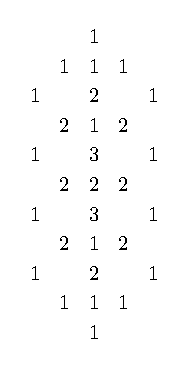
\includegraphics[width=1.7cm]{figures/E6.pdf}
			\vspace{2.9cm}
			\subcaption{$E_6$}
			}
			\parbox[t]{.15\textwidth}{\centering
			\vspace{0cm}
			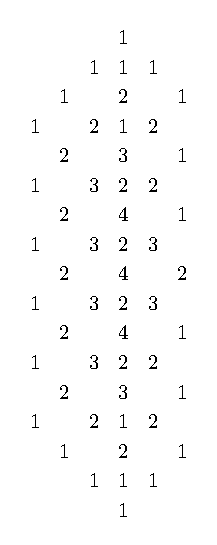
\includegraphics[width=1.7cm]{figures/E7.pdf}
			\vspace{1.95cm}
			\subcaption{$E_7$}
			}
			\parbox[t]{.15\textwidth}{\centering
			\vspace{0cm}
			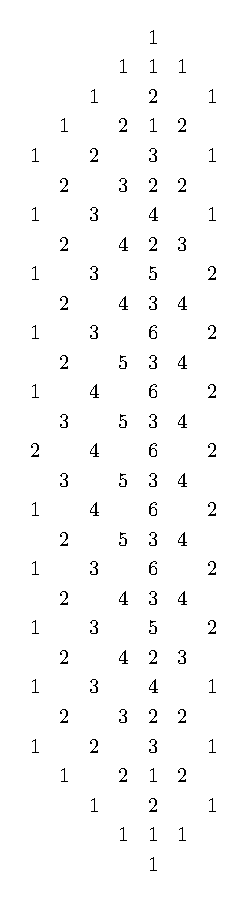
\includegraphics[width=1.7cm]{figures/E8.pdf}
			\subcaption{$E_8$}
			}
		\caption[Caption for LOF]{The quantity  $\orde$ for indecomposable representations in type $E$ arranged in the  Auslander--Reiten quiver.\footnotemark}
		\label{fig:startingfunction}
	\end{figure}
\end{center}
\footnotetext{Some representations $M$ are hidden when $\orde(M)=0$. In \cite{bongartz1984critical} the Figure \ref{fig:startingfunction} is called the starting functions.}

For an \textbf{indecomposable} quiver representation $M \in \rep(Q)$, we define the order of $M$ by
$$\ord(M):= \max_{i \in v(Q)} \dim_K M_i.$$
When the quiver $Q$ is of type $E$, we denote by $e \in v(Q)$ the unique vertex which is connected to three other vertices, and the number 
$$\orde(M):=\dim_K M_e=[P(e),M]$$
is equal to $\ord(M)$ unless $\orde(M)=0$.

The next lemma shows the affine paving property for representations of small order.

\begin{lemma}[{Follows \cite[Lemma 2.22]{maksimau2019flag}}]\label{lem:smallvecdim}
	Suppose that the underlying graph of $Q$ is a tree. For an indecomposable representation $M \in \rep(Q)$ with $\ord(M) \leqslant 2$, the variety $\Grr_{\dimvec{f}}(\Phi(M))$ is either empty or a direct product of some copies of $\mathbb{P}^1$. Especially, the partial flag variety $ \Grr_{\dimvec{f}}(\Phi(M))$ has an affine paving.
\end{lemma}
\begin{proof}\belowdisplayskip=-12pt
	For every $i \in v(Q)$, $\dim_K M_i\leqslant 2$. Since $Q$ is a tree and $M$ is indecomposable, for every $b\in a(Q)$ satisfying $\dim_K M_{s(b)}= \dim_K M_{t(b)}=2$, the map $M_{s(b)} \longrightarrow M_{t(b)}$ is an isomorphism. Therefore, when $\Grr_{\dimvec{f}}(\Phi(M)) \neq \varnothing$,\footnote{This condition imposes very strong restrictions on $\dimvec{f}$.} we get the natural embedding
	$$\Grr_{\dimvec{f}}(\Phi(M)) \longrightarrow \prod_{\substack{i \in v(Q) \;s.t.\\ \dim_K M_i=2 \\ \dimvec{f}_{(i,r)}=1 \text{ for some }r}} \mathbb{P}^1,$$\\[0.3cm]
	and the information of non-vertical arrows in the extended quiver (see Example \ref{eg:ext_quiver}) just reduce the number of $\mathbb{P}^1$. Precisely, one need to carefully discuss three cases of $M_i \longrightarrow M_j$:
	% https://q.uiver.app/?q=WzAsNyxbMCwwLCJLIl0sWzMsMCwiSyJdLFsxLDAsIkteMiJdLFsyLDAsIkteMiJdLFs1LDAsIkteMiJdLFs2LDAsIkteMi4iXSxbNCwwLCJcXHRleHR7YW5kfSJdLFs0LDUsIlxcY29uZyJdLFszLDEsIiIsMCx7InN0eWxlIjp7ImhlYWQiOnsibmFtZSI6ImVwaSJ9fX1dLFswLDIsIiIsMCx7InN0eWxlIjp7InRhaWwiOnsibmFtZSI6Imhvb2siLCJzaWRlIjoidG9wIn19fV1d
	\[\begin{tikzcd}
		K & {K^2} & {K^2} & K &[-0.5cm] {\text{and}} &[-0.5cm] {K^2} & {K^2.}
		\arrow["\cong", from=1-6, to=1-7]
		\arrow[two heads, from=1-3, to=1-4]
		\arrow[hook, from=1-1, to=1-2]
	\end{tikzcd}\]
\end{proof}

Now we've nearly prepared every step of the proof of Theorem \ref{thm:Dynkincase}. By following the process in Figure \ref{fig:flowchart}, we now prove Theorem \ref{thm:Dynkincase} assuming Claim \ref{claim:bigorder}. We will prove Claim \ref{claim:bigorder} in Appendix \ref{appendix:proofcomplement}.

\begin{figure}[ht]
    \centering
    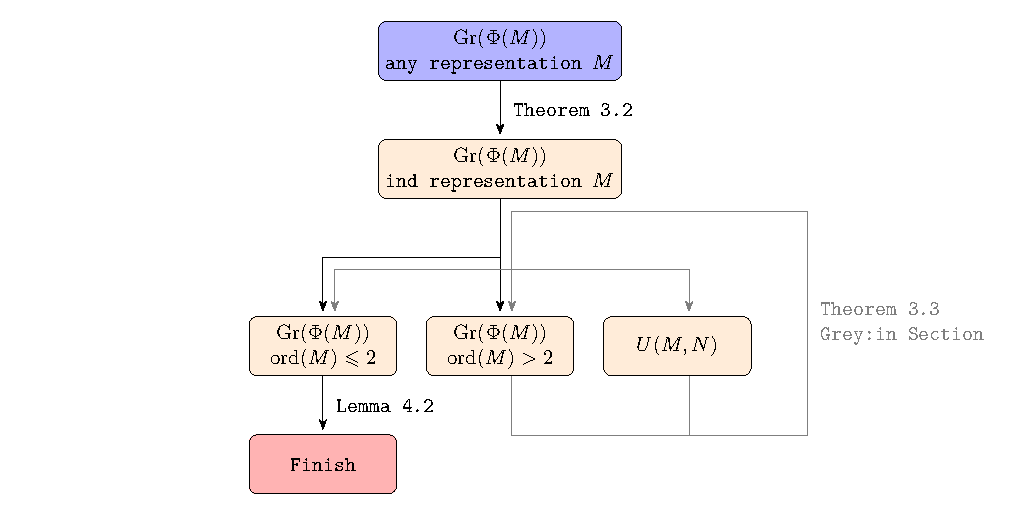
\includegraphics[scale=0.7]{figures/flowchart.pdf}
    \caption{the process of induction}
    \vspace{2mm}
    \label{fig:flowchart}
\end{figure}

\begin{claim}\label{claim:bigorder}
Suppose $Q$ is of Dynkin type. For any indecomposable representation $M \in \rep(Q)$ with $\ord(M)>2$, the (strict) partial flag variety $\Grr(\Phi(M))$ has an affine paving.
\end{claim}

\begin{proof}[{Proof of Theorem \ref{thm:Dynkincase}}]
First of all, for any indecomposable representation $M \in \rep(Q)$ we obtain an affine paving. This follows from Claim \ref{claim:bigorder} when $\ord(M)>2$, and follows from Lemma \ref{lem:smallvecdim} when $\ord(M)\leqslant 2$.

The general case follows by induction on the dimension vector. The indecomposable representations $\{N_i\}_{i \in Q_0}$ of quiver $Q$ can be ordered such that $[N_i,N_j]=0$ for all $i>j$. Therefore, every non-indecomposable representation $M$ can be decomposed as the direct sum of two nonzero representations $M_1, M_2$ satisfying $[M_2,M_1]^1=0$.
By applying Theorem \ref{thm:main1} to the short exact sequence 
$$0 \longrightarrow M_1 \longrightarrow M \longrightarrow M_2 \longrightarrow 0,$$
we get an affine paving from the affine pavings of $M_1$ and $M_2$, see Remark \ref{rem:topo}.
\end{proof}
\begin{remark}\label{rem:smallorder}
By the same technique one can show that, for Dynkin quiver $Q$ and any representation $M$ with $\displaystyle\max_{i \in v(Q)} \dim_K M_i \leqslant 2$, the variety $\Grr_{\dimvec{f}}(\Phi(M))$ has an affine paving. This result does not depend on Claim \ref{claim:bigorder}.
\end{remark}



%%%%%%%%%%%%%%%%%%%%%%%%%%%%%%%%%%%%%%%%%%%%%%%%%%%%%%%%%%%%%%%%%%%%%%%%%%%%%%%%%%%%%%%%%%%%%%%
\section{Application: Affine Case}\label{sec:affine}
This section tries to explain the difficulty of the Conjecture \ref{conj:affinecase}.

\begin{conj}\label{conj:affinecase}
For any affine quiver $Q$ and any indecomposable representation $M \in \rep(Q)$, the (strict) partial flag variety $\Flag{}(M)\cong\Grr(\Phi(M))$ has an affine paving.
\end{conj}

Actually, if readers follow the proof in \cite[Section 6]{irelli2019cell}, and change everything from $\Gr(-)$ to $\Grr(\Phi(-))$, then there is no difference except the Proposition 48, in which the authors proved the affine paving properties of quasi-simple regular representations. So we reduced the question to the case of quasi-simple regular representation. Combined with Lemma \ref{lem:affineADcase}, we've proved the affine paving properties for $\tilde{A},\tilde{D}$ cases.

\begin{lemma}\label{lem:affineADcase}
	Assume that $Q$ is a affine quiver of type $A$ or $D$, $M \in \rep(Q)$ is the \textbf{regular quasi-simple} representation, then the Grassmannian $\Grr(\Phi(M))$ has an affine paving.
\end{lemma}
\begin{proof}
The concept ``quasi-simple'' is defined in \cite[Definition 15]{irelli2019cell}; the concepts ``preprojective'',``preinjective'' and ``regular'' are defined in \cite[2.1.1]{irelli2019cell}. It's shown in \cite[Section 9, Lemma 3]{crawley1992lectures} that the regular quasi-simple representation $M$ have dimension vector smaller or equal to the minimal positive imaginary root, thus $\orde(M) \leqslant 2$ for the quiver of type $\tilde{D}$ and $\orde(M) \leqslant 1$ for the quiver of type $\tilde{A}$.
\end{proof}
%We use rep 2 Cor 18.8.

For a regular quasi-simple representation $Y$ of type $\tilde{E}$, it's possible that there's no short exact sequence
$$\eta:0\longrightarrow X \longrightarrow Y \longrightarrow S \longrightarrow 0$$
such that $[S,X]^1 \leqslant 1$. Then we can no longer use Theorem \ref{thm:main1} or \ref{thm:main2}. Hence, the new methods are needed for this case.
\appendix
%\setcounter{secnumdepth}{0}
%\section{Appendix}

\section{A crash course on Auslander--Reiten theory}\label{appendix:arth}

In this appendix, we will introduce concepts in Auslander--Reiten theory one by one: indecomposable representation, irreducible morphism, Auslander--Reiten translation, Auslander--Reiten sequence, Auslander--Reiten quiver, and minimal sectional mono. The main references for the material covered in this appendix are \cite{crawley1992lectures,maksimau2019flag}.

\begin{defn}[Indecomposable module]
Fix an algebra $R$. A non-zero module $M \in \mod(R)$ is called indecomposable if $M$ can not be written as a direct sum of two non-zero submodules. The set of all indecomposable modules is denoted by $\ind(R)$.
\end{defn}
There are several descriptions of the indecomposable representations in special cases. For instance:
\begin{itemize}
\item By Gabriel's theorem \cite[Theorem  2.1]{article}, the functor $\dimv$ yields a bijection from the indecomposable representations of a Dynkin quiver to the positive roots of the associated Lie algebra.

There is a unique indecomposable representation of maximal dimension vector which corresponds to the unique maximal positive root. This is shown in Table \ref{table:importantroots}.

\item By \cite[Theorem 2, p34]{crawley1992lectures}, in the affine case, the functor $\dimv$ yields a surjective map from the indecomposable representations to the positive roots of the associated affine diagram. The map is $\infty$-to-$1$ when the root is imaginary, and is $1$-to-$1$ when the root is real.\footnote{The root $\alpha \in \dimv(Q)$ is called real if $\left< \alpha,\alpha \right>=1$, and called imaginary if $\left< \alpha,\alpha \right>=0$.}
%See Jan's lecture notes about Theorem 11.4(Kac)

We also have a unique minimal imaginary root $\delta$ which controls the whole indecomposable representation theory, as shown in Table \ref{table:importantroots}.

\item All indecomposable representations of Dynkin quivers and all indecomposable representations of affine quivers corresponding to the positive real roots $\alpha$ with $\alpha < \delta$ or $\left< \alpha,\delta \right> \neq 0$ are rigid, i.e., $[M,M]^1=0$. They are also bricks, i.e., $[M,M]^1=0$ and $[M,M]=1$.\footnote{Any rigid indecomposable module of a hereditary algebra is a brick.}
%This is a result coming from Jan Cor 15.2
% Sadly, not every indecomposable representation of affine quivers have $[M,M]=1$, see https://math.stackexchange.com/questions/966646/endomorphism-ring-of-indecomposable-representations.
\end{itemize}

\renewcommand{\arraystretch}{1.2}
\begin{table}
\centering
\begin{tabular}{|c|c|c|}
\hline
Type & maximal positive real root(Dynkin) & minimal positive imaginary root $\delta$(affine) \\
\hline
$A$ & \begin{tikzcd}[sep=4mm]
	&& {} \\
	1 & 1 & \cdots & 1 & 1
	\arrow[no head, from=2-1, to=2-2]
	\arrow[no head, from=2-2, to=2-3]
	\arrow[no head, from=2-3, to=2-4]
	\arrow[no head, from=2-4, to=2-5]
\end{tikzcd} &
\begin{tikzcd}[sep=4mm]
	&& 1 \\
	1 & 1 & \cdots & 1 & 1
	\arrow[no head, from=2-1, to=2-2]
	\arrow[no head, from=2-2, to=2-3]
	\arrow[no head, from=2-3, to=2-4]
	\arrow[no head, from=2-4, to=2-5]
	\arrow[no head, from=2-1, to=1-3]
	\arrow[no head, from=1-3, to=2-5]
\end{tikzcd}
  \\
\hline
$D$ & \begin{tikzcd}[sep=4mm]
	&&& 1 \\
	1 & 1 & \cdots & 2 & 1
	\arrow[no head, from=2-1, to=2-2]
	\arrow[no head, from=2-2, to=2-3]
	\arrow[no head, from=2-3, to=2-4]
	\arrow[no head, from=2-4, to=2-5]
	\arrow[no head, from=1-4, to=2-4]
\end{tikzcd} &
\begin{tikzcd}[sep=4mm]
	& 1 && 1 \\
	1 & 2 & \cdots & 2 & 1
	\arrow[no head, from=2-1, to=2-2]
	\arrow[no head, from=2-2, to=2-3]
	\arrow[no head, from=2-3, to=2-4]
	\arrow[no head, from=2-4, to=2-5]
	\arrow[no head, from=1-4, to=2-4]
	\arrow[no head, from=1-2, to=2-2]
\end{tikzcd}
  \\
\hline
$E_6$ &\begin{tikzcd}[sep=4mm]
	&& 2 \\
	1 & 2 & 3 & 2 & 1
	\arrow[no head, from=2-1, to=2-2]
	\arrow[no head, from=2-2, to=2-3]
	\arrow[no head, from=2-3, to=2-4]
	\arrow[no head, from=2-4, to=2-5]
	\arrow[no head, from=1-3, to=2-3]
\end{tikzcd}  & 
\begin{tikzcd}[sep=4mm]
	& 1 & 2 \\
	1 & 2 & 3 & 2 & 1
	\arrow[no head, from=2-1, to=2-2]
	\arrow[no head, from=2-2, to=2-3]
	\arrow[no head, from=2-3, to=2-4]
	\arrow[no head, from=2-4, to=2-5]
	\arrow[no head, from=1-3, to=2-3]
	\arrow[no head, from=1-2, to=1-3]
\end{tikzcd} \\
\hline
$E_7$ & \begin{tikzcd}[sep=4mm]
	&&& 2 \\
	1 & 2 & 3 & 4 & 3 & 2
	\arrow[no head, from=2-2, to=2-3]
	\arrow[no head, from=2-3, to=2-4]
	\arrow[no head, from=2-4, to=2-5]
	\arrow[no head, from=2-5, to=2-6]
	\arrow[no head, from=1-4, to=2-4]
	\arrow[no head, from=2-1, to=2-2]
\end{tikzcd}
 &
 \begin{tikzcd}[sep=4mm]
 	&&& 2 \\
 	1 & 2 & 3 & 4 & 3 & 2 & 1
 	\arrow[no head, from=2-2, to=2-3]
 	\arrow[no head, from=2-3, to=2-4]
 	\arrow[no head, from=2-4, to=2-5]
 	\arrow[no head, from=2-5, to=2-6]
 	\arrow[no head, from=1-4, to=2-4]
 	\arrow[no head, from=2-1, to=2-2]
 	\arrow[no head, from=2-6, to=2-7]
 \end{tikzcd}  \\
\hline
$E_8$ & \begin{tikzcd}[sep=4mm]
	&&&& 3 \\
	2 & 3 & 4 & 5 & 6 & 4 & 2
	\arrow[no head, from=2-3, to=2-4]
	\arrow[no head, from=2-4, to=2-5]
	\arrow[no head, from=2-5, to=2-6]
	\arrow[no head, from=2-6, to=2-7]
	\arrow[no head, from=1-5, to=2-5]
	\arrow[no head, from=2-2, to=2-3]
	\arrow[no head, from=2-1, to=2-2]
\end{tikzcd} & 
\begin{tikzcd}[sep=4mm]
	&&&&& 3 \\
	1 & 2 & 3 & 4 & 5 & 6 & 4 & 2
	\arrow[no head, from=2-4, to=2-5]
	\arrow[no head, from=2-5, to=2-6]
	\arrow[no head, from=2-6, to=2-7]
	\arrow[no head, from=2-7, to=2-8]
	\arrow[no head, from=1-6, to=2-6]
	\arrow[no head, from=2-3, to=2-4]
	\arrow[no head, from=2-2, to=2-3]
	\arrow[no head, from=2-1, to=2-2]
\end{tikzcd}
\\
\hline
\end{tabular}
\vspace{1mm}
\caption{Roots which control all other roots.}
\label{table:importantroots}
\end{table}
Indecomposable representations form the vertices of Auslander–Reiten quiver, while irreducible morphisms form the arrows.
\begin{defn}[Irreducible morphism]
Given two indecomposable representations $T,T' \in \Mod(R)$, denote
\begin{equation*}
\begin{aligned}
  \rad(T,T'):=\;& \left\{ f \in \Hom_{R}(T,T')  \middle|  f \text{ is not invertible}  \right\} \\
  =\;& \begin{cases}
  \Hom_{R}(T,T') & T \ncong T',\\
  \Jac(\End_R(T)) & T \cong T'.
  \end{cases} 
\end{aligned}
\end{equation*}
be the radical, and let
$$\rad^2(T,T'):= \bigcup_{S \in \ind(R)} \Img \big[ \rad(T,S) \times \rad(S,T') \longrightarrow \rad(T,T')  \big]$$
be the subspace of $\rad(T,T')$. A morphism $f\in \Hom_{R}(T,T')$ is called irreducible if $f \in \rad(T,T') \setminus \rad^2(T,T')$.
\end{defn}

The definition of irreducible morphism applies to any representation, and one can easily show that any irreducible morphism is either injective or surjective.

\begin{defn}\label{def:Auslander--Reiten translation}
Let $R=KQ/I$ be a bounded quiver algebra. We define the Nakayama functor $\nu_R$, Auslander--Reiten translation $\tau_R$, and inverse Auslander--Reiten translation $\tau_R^{-1}$, as follows:
% https://q.uiver.app/?q=WzAsMTIsWzAsMCwiXFxudV9SOiJdLFsxLDAsIlxcTW9kKFIpIl0sWzMsMCwiXFxNb2QoUikiXSxbMiwwLCJcXE1vZChSXntvcH0pIl0sWzEsMSwiXFxNb2Rkb3duKFIpIl0sWzMsMSwiXFxNb2R1cChSKSJdLFsyLDEsIlxcTW9kZG93bihSXntvcH0pIl0sWzAsMSwiXFx0YXVfUjoiXSxbMCwyLCJcXHRhdV9SXnstMX06Il0sWzMsMiwiXFxNb2Rkb3duKFIpIl0sWzIsMiwiXFxNb2Rkb3duKFJee29wfSkiXSxbMSwyLCJcXE1vZHVwKFIpIl0sWzEsMywiXFxIb21fUigtLF9SXFwhUikiXSxbMywyLCJcXEhvbV9LKC0sSykiXSxbNCw2LCJcXEV4dF4xX1IoLSxfUlxcIVIpIl0sWzYsNSwiXFxIb21fSygtLEspIl0sWzExLDEwLCJcXEhvbV9LKC0sSykiXSxbMTAsOSwiXFxFeHReMV97Ul57b3B9fSgtLFJfUikiXV0=
\[\begin{tikzcd}[row sep=0mm, column sep=2cm]
	{\nu_R:} &[-1.8cm] {\Mod(R)} & {\Mod(R^{op})} & {\Mod(R)}, \\
	{\tau_R:} & {\Moddown(R)} & {\Moddown(R^{op})} & {\Modup(R)}, \\
	{\tau_R^{-1}:} & {\Modup(R)} & {\Moddown(R^{op})} & {\Moddown(R)}.
	\arrow["{\Hom_R(-,_R\!R)}", from=1-2, to=1-3]
	\arrow["{\Hom_K(-,K)}", from=1-3, to=1-4]
	\arrow["{\Ext^1_R(-,_R\!R)}", from=2-2, to=2-3]
	\arrow["{\Hom_K(-,K)}", from=2-3, to=2-4]
	\arrow["{\Hom_K(-,K)}", from=3-2, to=3-3]
	\arrow["{\Ext^1_{R^{op}}(-,R_R)}", from=3-3, to=3-4]
\end{tikzcd}\]
Here $\Moddown(R)$ and $\Modup(R)$ denote the stable module categories. The objects are the same as in $\Mod(R)$, and their morphisms are modified by ``collapsing'' the morphisms passing through projective/injective modules to zero, i.e.,
\begin{equation*}
\begin{aligned}
  \Mor_{\Moddown(R)}(T,T'):=\;& \Mor_{\Mod(R)}(T,T')/(f:T \rightarrow P \rightarrow T', P \text{ is projective}), \\ 
  \Mor_{\Modup(R)}(T,T'):=\;& \Mor_{\Mod(R)}(T,T')/(f:T \rightarrow I \rightarrow T', I \text{ is injective}).
\end{aligned}
\end{equation*}
These modifications guarantee that the Auslander--Reiten translation $\tau_R$ is indeed a functor. For convenience, we abbreviate $\Mor_{\Moddown(R)}$, $\Mor_{\Modup(R)}$, $\Mor_{\Mod(R)}$ as $\Homdown_R$, $\Homup_R$, $\Hom_R$, and ignore the subscription $R$ in the symbol $\tau_R$.
\end{defn}
The Auslander--Reiten translation has many magical properties. For example, $\tau_R$ induces the one-to-one correspondence between non-projective indecomposable representations and non-injective indecomposable representations. We would also frequently use the Auslander--Reiten formulas: ($(-)^{\vee}=\Hom_K(-,K)$ is the dual)
$$\left(\Homup_R (T,\tau T') \right)^{\vee} \stackrel{\sim}{\longrightarrow} \Ext_R^1(T',T)$$
$$\left(\Homdown_R (\tau^{-1}T,T') \right)^{\vee} \stackrel{\sim}{\longrightarrow} \Ext_R^1(T',T)$$
which is functorial for any $T,T' \in \Mod(R)$. Especially, when $T$ is not injective, $\Homup_R (T,\tau T')=\Hom_R (T,\tau T')$, we get $[T',T]^1=[T,\tau T']$; when $T'$ is not projective, $\Homdown_R (\tau^{-1}T,T')=\Hom_R (\tau^{-1}T,T')$, we get $[T',T]^1=[\tau^{-1}T, T']$.

For the Auslander–Reiten sequence there can be many equivalent definitions, and we only present one due to limitations of space. 
\begin{defn}[Auslander–Reiten sequence]
For $X \in \ind (R)$ non-projective, an epimorphism $g:E \longrightarrow X$ is called \textbf{right almost split} if $g$ is not split epi and every homomorphism $h:T \longrightarrow X$ which is not split epi factors through $E$. The short exact sequence 
$$0 \longrightarrow \tau X \longrightarrow E \stackrel{g}{\longrightarrow} X \longrightarrow 0$$
is called an Auslander–Reiten sequence if $g$ is right almost split.
\end{defn}

All the concepts introduced in this appendix can be clearly observed from the Auslander–Reiten quiver. In the Auslander–Reiten quiver the vertices are indecomposable representations, the arrows are irreducible morphisms among indecomposable representations, Auslander--Reiten translation is labeled as the dotted arrow, and the Auslander–Reiten sequence can be read by collecting all paths from $\tau X$ to $X$. For instance, in Figure \ref{fig:Auslander–Reiten_quiver} we can get an Auslander–Reiten sequence 
\renewcommand{\arraystretch}{0.5}
$$0 \longrightarrow \begin{matrix}
2\\
12321
\end{matrix} \longrightarrow
\begin{matrix}
1\\
12211
\end{matrix} \oplus
\begin{matrix}
1\\
11110
\end{matrix} \oplus
\begin{matrix}
1\\
01221
\end{matrix}
 \longrightarrow
\begin{matrix}
1\\
12221
\end{matrix} \longrightarrow
0
$$
\renewcommand{\arraystretch}{1}
of the corresponding quiver.

%https://www.math.uni-bielefeld.de/~wcrawley/knitting/?projectives=1:,2:1+3,3:,4:3,5:43,6:3&orientation=vertical&positions=1:(500|0),2:(400|0),3:(300|0),4:(200|0),5:(100|0),6:(320|0)

% https://q.uiver.app/?q=WzAsMzYsWzAsMCwiXFxzdWJzdGFja3swXFxcXDEwMDAwfSJdLFszLDAsIlxcc3Vic3RhY2t7MFxcXFwwMDEwMH0iXSxbMSwxLCJcXHN1YnN0YWNrezBcXFxcMTExMDB9Il0sWzIsMSwiXFxzdWJzdGFja3sxXFxcXDAwMTAwfSJdLFs0LDEsIlxcc3Vic3RhY2t7MFxcXFwwMDExMH0iXSxbMCwyLCJcXHN1YnN0YWNrezBcXFxcMDExMDB9Il0sWzMsMiwiXFxzdWJzdGFja3sxXFxcXDExMjEwfSJdLFs1LDIsIlxcc3Vic3RhY2t7MFxcXFwwMDExMX0iXSxbMSwzLCJcXHN1YnN0YWNrezFcXFxcMDEyMTB9Il0sWzIsMywiXFxzdWJzdGFja3swXFxcXDExMTEwfSJdLFs0LDMsIlxcc3Vic3RhY2t7MVxcXFwxMTIxMX0iXSxbMCw0LCJcXHN1YnN0YWNrezFcXFxcMDAxMTB9Il0sWzMsNCwiXFxzdWJzdGFja3sxXFxcXDEyMzIxfSJdLFs1LDQsIlxcc3Vic3RhY2t7MVxcXFwxMTEwMH0iXSxbMSw1LCJcXHN1YnN0YWNrezFcXFxcMTEyMjF9Il0sWzIsNSwiXFxzdWJzdGFja3sxXFxcXDAxMjExfSJdLFs0LDUsIlxcc3Vic3RhY2t7MVxcXFwxMjIxMH0iXSxbMCw2LCJcXHN1YnN0YWNrezBcXFxcMTExMTF9Il0sWzMsNiwiXFxzdWJzdGFja3syXFxcXDEyMzIxfSJdLFs1LDYsIlxcc3Vic3RhY2t7MFxcXFwwMTExMH0iXSxbMSw3LCJcXHN1YnN0YWNrezFcXFxcMTIyMTF9Il0sWzIsNywiXFxzdWJzdGFja3sxXFxcXDExMTEwfSJdLFs0LDcsIlxcc3Vic3RhY2t7MVxcXFwwMTIyMX0iXSxbMCw4LCJcXHN1YnN0YWNrezFcXFxcMDExMDB9Il0sWzAsMTAsIlxcc3Vic3RhY2t7MFxcXFwwMDAxMH0iXSxbMCwxMiwiXFxzdWJzdGFja3swXFxcXDAwMDAxfSJdLFsxLDExLCJcXHN1YnN0YWNrezBcXFxcMDAwMTF9Il0sWzIsMTEsIlxcc3Vic3RhY2t7MVxcXFwwMDAwMH0iXSxbNCwxMSwiXFxzdWJzdGFja3swXFxcXDAxMDAwfSJdLFszLDEwLCJcXHN1YnN0YWNrezFcXFxcMDExMTF9Il0sWzUsMTAsIlxcc3Vic3RhY2t7MFxcXFwxMTAwMH0iXSxbMSw5LCJcXHN1YnN0YWNrezFcXFxcMDExMTB9Il0sWzIsOSwiXFxzdWJzdGFja3swXFxcXDAxMTExfSJdLFs0LDksIlxcc3Vic3RhY2t7MVxcXFwxMTExMX0iXSxbMyw4LCJcXHN1YnN0YWNrezFcXFxcMTIyMjF9Il0sWzUsOCwiXFxzdWJzdGFja3sxXFxcXDAwMTExfSJdLFswLDJdLFsxLDJdLFsxLDNdLFsxLDRdLFsyLDVdLFsyLDZdLFszLDZdLFs0LDZdLFs0LDddLFs3LDEwXSxbNiwxMF0sWzYsOV0sWzYsOF0sWzUsOF0sWzgsMTFdLFs4LDEyXSxbOSwxMl0sWzEwLDEyXSxbMTAsMTNdLFsxMywxNl0sWzEyLDE2XSxbMTIsMTVdLFsxMiwxNF0sWzExLDE0XSxbMTQsMTddLFsxNCwxOF0sWzE1LDE4XSxbMTYsMThdLFsxNiwxOV0sWzE3LDIwXSxbMTgsMjBdLFsxOCwyMV0sWzE4LDIyXSxbMTksMjJdLFsyMiwzNV0sWzIyLDM0XSxbMjEsMzRdLFsyMCwzNF0sWzIwLDIzXSxbMjMsMzFdLFszNCwzMV0sWzM0LDMyXSxbMzQsMzNdLFszNSwzM10sWzMzLDMwXSxbMzMsMjldLFszMiwyOV0sWzMxLDI5XSxbMzEsMjRdLFsyNCwyNl0sWzI5LDI2XSxbMjksMjddLFsyOSwyOF0sWzMwLDI4XSxbMjYsMjVdLFs1LDAsIiIsMSx7InN0eWxlIjp7ImJvZHkiOnsibmFtZSI6ImRhc2hlZCJ9fX1dLFs2LDEsIiIsMSx7InN0eWxlIjp7ImJvZHkiOnsibmFtZSI6ImRhc2hlZCJ9fX1dLFs4LDIsIiIsMSx7InN0eWxlIjp7ImJvZHkiOnsibmFtZSI6ImRhc2hlZCJ9fX1dLFs5LDMsIiIsMSx7InN0eWxlIjp7ImJvZHkiOnsibmFtZSI6ImRhc2hlZCJ9fX1dLFsxMCw0LCIiLDEseyJzdHlsZSI6eyJib2R5Ijp7Im5hbWUiOiJkYXNoZWQifX19XSxbMTEsNSwiIiwxLHsic3R5bGUiOnsiYm9keSI6eyJuYW1lIjoiZGFzaGVkIn19fV0sWzEyLDYsIiIsMSx7InN0eWxlIjp7ImJvZHkiOnsibmFtZSI6ImRhc2hlZCJ9fX1dLFsxMyw3LCIiLDEseyJzdHlsZSI6eyJib2R5Ijp7Im5hbWUiOiJkYXNoZWQifX19XSxbMTQsOCwiIiwxLHsic3R5bGUiOnsiYm9keSI6eyJuYW1lIjoiZGFzaGVkIn19fV0sWzE1LDksIiIsMSx7InN0eWxlIjp7ImJvZHkiOnsibmFtZSI6ImRhc2hlZCJ9fX1dLFsxNiwxMCwiIiwxLHsic3R5bGUiOnsiYm9keSI6eyJuYW1lIjoiZGFzaGVkIn19fV0sWzE5LDEzLCIiLDEseyJzdHlsZSI6eyJib2R5Ijp7Im5hbWUiOiJkYXNoZWQifX19XSxbMTgsMTIsIiIsMSx7InN0eWxlIjp7ImJvZHkiOnsibmFtZSI6ImRhc2hlZCJ9fX1dLFsxNywxMSwiIiwxLHsic3R5bGUiOnsiYm9keSI6eyJuYW1lIjoiZGFzaGVkIn19fV0sWzIwLDE0LCIiLDEseyJzdHlsZSI6eyJib2R5Ijp7Im5hbWUiOiJkYXNoZWQifX19XSxbMjEsMTUsIiIsMSx7InN0eWxlIjp7ImJvZHkiOnsibmFtZSI6ImRhc2hlZCJ9fX1dLFsyMiwxNiwiIiwxLHsic3R5bGUiOnsiYm9keSI6eyJuYW1lIjoiZGFzaGVkIn19fV0sWzIzLDE3LCIiLDEseyJzdHlsZSI6eyJib2R5Ijp7Im5hbWUiOiJkYXNoZWQifX19XSxbMzQsMTgsIiIsMSx7InN0eWxlIjp7ImJvZHkiOnsibmFtZSI6ImRhc2hlZCJ9fX1dLFszNSwxOSwiIiwxLHsic3R5bGUiOnsiYm9keSI6eyJuYW1lIjoiZGFzaGVkIn19fV0sWzMzLDIyLCIiLDEseyJzdHlsZSI6eyJib2R5Ijp7Im5hbWUiOiJkYXNoZWQifX19XSxbMzEsMjAsIiIsMSx7InN0eWxlIjp7ImJvZHkiOnsibmFtZSI6ImRhc2hlZCJ9fX1dLFszMiwyMSwiIiwxLHsic3R5bGUiOnsiYm9keSI6eyJuYW1lIjoiZGFzaGVkIn19fV0sWzI0LDIzLCIiLDEseyJzdHlsZSI6eyJib2R5Ijp7Im5hbWUiOiJkYXNoZWQifX19XSxbMjUsMjQsIiIsMSx7InN0eWxlIjp7ImJvZHkiOnsibmFtZSI6ImRhc2hlZCJ9fX1dLFsyNiwzMSwiIiwxLHsic3R5bGUiOnsiYm9keSI6eyJuYW1lIjoiZGFzaGVkIn19fV0sWzI3LDMyLCIiLDEseyJzdHlsZSI6eyJib2R5Ijp7Im5hbWUiOiJkYXNoZWQifX19XSxbMjksMzQsIiIsMSx7InN0eWxlIjp7ImJvZHkiOnsibmFtZSI6ImRhc2hlZCJ9fX1dLFsyOCwzMywiIiwxLHsic3R5bGUiOnsiYm9keSI6eyJuYW1lIjoiZGFzaGVkIn19fV0sWzMwLDM1LCIiLDEseyJzdHlsZSI6eyJib2R5Ijp7Im5hbWUiOiJkYXNoZWQifX19XV0=

\begin{figure}[ht]
  \vspace{0cm}
    \centering  \[\begin{tikzcd}[row sep=5mm]
    	{\substack{0\\10000}} &&[-5mm]&[-16mm] {\substack{0\\00100}} \\
    	& {\substack{0\\11100}} & {\substack{1\\00100}} && {\substack{0\\00110}} \\
    	{\substack{0\\01100}} &&& {\substack{1\\11210}} && {\substack{0\\00111}} \\
    	& {\substack{1\\01210}} & {\substack{0\\11110}} && {\substack{1\\11211}} \\
    	{\substack{1\\00110}} &&& {\substack{1\\12321}} && {\substack{1\\11100}} \\
    	& {\substack{1\\11221}} & {\substack{1\\01211}} && {\substack{1\\12210}} \\
    	{\substack{0\\11111}} &&& {\substack{2\\12321}} && {\substack{0\\01110}} \\
    	& {\substack{1\\12211}} & {\substack{1\\11110}} && {\substack{1\\01221}} \\
    	{\substack{1\\01100}} &&& {\substack{1\\12221}} && {\substack{1\\00111}} \\
    	& {\substack{1\\01110}} & {\substack{0\\01111}} && {\substack{1\\11111}} \\
    	{\substack{0\\00010}} &&& {\substack{1\\01111}} && {\substack{0\\11000}} \\
    	& {\substack{0\\00011}} & {\substack{1\\00000}} && {\substack{0\\01000}} \\
    	{\substack{0\\00001}}
    	\arrow[from=1-1, to=2-2]
    	\arrow[from=1-4, to=2-2]
    	\arrow[from=1-4, to=2-3]
    	\arrow[from=1-4, to=2-5]
    	\arrow[from=2-2, to=3-1]
    	\arrow[from=2-2, to=3-4]
    	\arrow[from=2-3, to=3-4]
    	\arrow[from=2-5, to=3-4]
    	\arrow[from=2-5, to=3-6]
    	\arrow[from=3-6, to=4-5]
    	\arrow[from=3-4, to=4-5]
    	\arrow[from=3-4, to=4-3]
    	\arrow[from=3-4, to=4-2]
    	\arrow[from=3-1, to=4-2]
    	\arrow[from=4-2, to=5-1]
    	\arrow[from=4-2, to=5-4]
    	\arrow[from=4-3, to=5-4]
    	\arrow[from=4-5, to=5-4]
    	\arrow[from=4-5, to=5-6]
    	\arrow[from=5-6, to=6-5]
    	\arrow[from=5-4, to=6-5]
    	\arrow[from=5-4, to=6-3]
    	\arrow[from=5-4, to=6-2]
    	\arrow[from=5-1, to=6-2]
    	\arrow[from=6-2, to=7-1]
    	\arrow[from=6-2, to=7-4]
    	\arrow[from=6-3, to=7-4]
    	\arrow[from=6-5, to=7-4]
    	\arrow[from=6-5, to=7-6]
    	\arrow[from=7-1, to=8-2]
    	\arrow[from=7-4, to=8-2]
    	\arrow[from=7-4, to=8-3]
    	\arrow[from=7-4, to=8-5]
    	\arrow[from=7-6, to=8-5]
    	\arrow[from=8-5, to=9-6]
    	\arrow[from=8-5, to=9-4]
    	\arrow[from=8-3, to=9-4]
    	\arrow[from=8-2, to=9-4]
    	\arrow[from=8-2, to=9-1]
    	\arrow[from=9-1, to=10-2]
    	\arrow[from=9-4, to=10-2]
    	\arrow[from=9-4, to=10-3]
    	\arrow[from=9-4, to=10-5]
    	\arrow[from=9-6, to=10-5]
    	\arrow[from=10-5, to=11-6]
    	\arrow[from=10-5, to=11-4]
    	\arrow[from=10-3, to=11-4]
    	\arrow[from=10-2, to=11-4]
    	\arrow[from=10-2, to=11-1]
    	\arrow[from=11-1, to=12-2]
    	\arrow[from=11-4, to=12-2]
    	\arrow[from=11-4, to=12-3]
    	\arrow[from=11-4, to=12-5]
    	\arrow[from=11-6, to=12-5]
    	\arrow[from=12-2, to=13-1]
    	\arrow[dashed, from=3-1, to=1-1]
    	\arrow[dashed, from=3-4, to=1-4]
    	\arrow[dashed, from=4-2, to=2-2]
    	\arrow[dashed, from=4-3, to=2-3]
    	\arrow[dashed, from=4-5, to=2-5]
    	\arrow[dashed, from=5-1, to=3-1]
    	\arrow[dashed, from=5-4, to=3-4]
    	\arrow[dashed, from=5-6, to=3-6]
    	\arrow[dashed, from=6-2, to=4-2]
    	\arrow[dashed, from=6-3, to=4-3]
    	\arrow[dashed, from=6-5, to=4-5]
    	\arrow[dashed, from=7-6, to=5-6]
    	\arrow[dashed, from=7-4, to=5-4]
    	\arrow[dashed, from=7-1, to=5-1]
    	\arrow[dashed, from=8-2, to=6-2]
    	\arrow[dashed, from=8-3, to=6-3]
    	\arrow[dashed, from=8-5, to=6-5]
    	\arrow[dashed, from=9-1, to=7-1]
    	\arrow[dashed, from=9-4, to=7-4]
    	\arrow[dashed, from=9-6, to=7-6]
    	\arrow[dashed, from=10-5, to=8-5]
    	\arrow[dashed, from=10-2, to=8-2]
    	\arrow[dashed, from=10-3, to=8-3]
    	\arrow[dashed, from=11-1, to=9-1]
    	\arrow[dashed, from=13-1, to=11-1]
    	\arrow[dashed, from=12-2, to=10-2]
    	\arrow[dashed, from=12-3, to=10-3]
    	\arrow[dashed, from=11-4, to=9-4]
    	\arrow[dashed, from=12-5, to=10-5]
    	\arrow[dashed, from=11-6, to=9-6]
    \end{tikzcd}\]
    \caption{The Auslander–Reiten quiver of the quiver}
    \begin{tikzcd}[row sep=3mm, column sep=5mm]
    	                                &                 & \bullet \arrow[d] &                 &                 \\
 E_6:\bullet  & \bullet \arrow[r]\arrow[l] & \bullet           & \bullet \arrow[l] & \bullet \arrow[l]
    	\end{tikzcd}
     \label{fig:Auslander–Reiten_quiver}   
\end{figure} 
Finally we move forward to the definition of minimal sectional mono. The rest can be skipped until Lemma \ref{lem:msm&order}.

\begin{defn}[Sectional morphism]
Let $Q$ be a quiver of Dynkin/affine type, and $M,N \in \rep(Q)$ be two indecomposable representations of $Q$, which are preprojective\footnote{A representation $M \in \rep(Q)$ is called preprojective if $\tau^k M$ is projective for some $k \geqslant 0$. Similarly, A representation $M \in \rep(Q)$ is called preinjective if $\tau^{-k} M$ is injective for some $k \geqslant 0$.} when $Q$ is affine. A morphism $f \in \Hom_{KQ}(M,N)$ is called sectional if $f$ can be written as the composition
$$f: M=X_0 \stackrel{f_1}{\longrightarrow} X_1 \stackrel{f_2}{\longrightarrow} \cdots \stackrel{f_{t-1}}{\longrightarrow} X_{t-1} \stackrel{f_t}{\longrightarrow} X_t=N$$
where $f_i \in \Hom_{KQ}(X_{i-1},X_i)$ are irreducible morphisms between indecomposable representations, and $\tau X_{i+2} \ncong X_i$ for any suitable $i$.
\end{defn}
\begin{remark}
Let $f$ be a sectional morphism. If the underlying quiver $Q$ is a Dynkin/affine quiver without oriented cycles, then $X_0,\ldots,X_t$ are uniquely determined, and $f_1,\ldots, f_t$ are unique up to constant.
\end{remark}
\begin{lemma}
Any sectional morphism $f \in \Hom_{KQ}(M,N)$ is either surjective or injective.
\end{lemma}
\begin{proof}
When $Q$ is a quiver without oriented cycles, then $[N,M]^1 \leqslant [M,\tau N]=0$, thus by \cite[Lemma 7]{maksimau2019flag} we get the result; when $Q$ is of type $\tilde{A}$, the result comes from \cite[Lemma 51]{maksimau2019flag}.
\end{proof}
\begin{defn}[Sectional mono, minimal sectional mono]
Let $Q$ be a quiver without oriented cycles. A sectional morphism $f \in \Hom_{KQ}(M,N)$ is called as a sectional mono if $f$ is injective; a sectional mono is called minimal if $f_t \circ \cdots \circ f_{i+1}:X_i \longrightarrow N$ are surjective for any $i \in \{1,2,\ldots,t \}$.
\end{defn}
Minimal sectional monos can also be clearly seen from the Auslander–Reiten quiver, and we can check if a sectional morphism is mono by comparing the dimension vectors. In the case of Example $E_6$ in Figure \ref{fig:Auslander–Reiten_quiver}, a non-zero morphism from $\substack{1\\00110}$ to $\substack{1\\11110}$ is a minimal sectional mono while a non-zero morphism from $\substack{0\\01100}$ to $\substack{1\\01211}$ is not, since a sectional morphism from $\substack{1\\01210}$ to $\substack{1\\01211}$ is also injective.

\section{Proof of Claim \ref{claim:bigorder}}\label{appendix:proofcomplement}

The task of this appendix is to prove Claim \ref{claim:bigorder}. When the quiver $Q$ is of type $A$ or $D$, Claim \ref{claim:bigorder} is trivially true since no indecomposable representation can have order bigger than two. So we only concentrate on type $E$.

The idea of the proof is as follows. For any indecomposable representation $Y$ with $\ord(Y)>2$, we put $Y$ into a short exact sequence 
$$\eta:0\longrightarrow X \longrightarrow Y \longrightarrow S \longrightarrow 0$$
fulfilling the assumptions of Theorem \ref{thm:main2}, and then $\Gr(\Phi(Y))$ has an affine paving if $\Img \Psi$ has. If additionally the map $X \hookrightarrow Y$ is a minimal sectional mono, then $\Img \Psi_{f,g}$ can be written as the product space, which makes $\Img \Psi$ easier to understand.




\begin{center}
    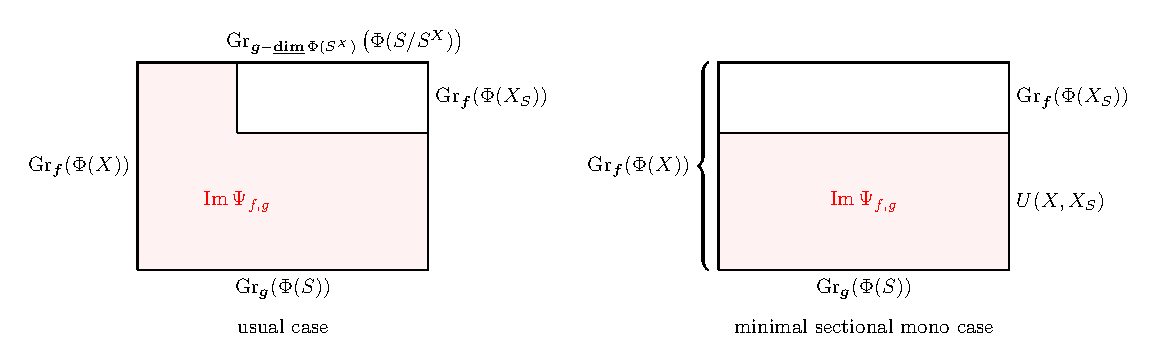
\includegraphics[scale=0.7]{figures/preferredimage.pdf}
\end{center}

The next two lemmas tell us the existence of the desired short exact sequence.
\begin{lemma}\label{lem:msm&order}
	For every indecomposable representation $Y$ of type $E$ with $\ord(Y)>2$, there is a minimal sectional mono $f:X \longrightarrow Y$.
\end{lemma}
\begin{proof}
	Just observe the Auslander--Reiten quiver. The chosen minimal sectional monos are represented in Figure \ref{fig:minisecmono}. Notice that for the most time $\orde(-)$ is enough to guarantee the map to be a mono.
\end{proof}
	\begin{center}
		\begin{figure}[ht]
			\vspace{0cm}
			\parbox[t]{.15\textwidth}{\centering
			\vspace{0cm}
			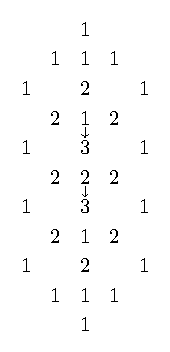
\includegraphics[width=1.7cm]{figures/E6easy.pdf}
			\vspace{4.14cm}
			\subcaption{$E_6$}
			}
			\parbox[t]{.20\textwidth}{\centering
			\vspace{0cm}
			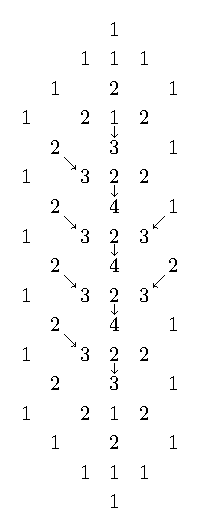
\includegraphics[width=1.7cm]{figures/E7easy.pdf}
			\vspace{3.17cm}
			\subcaption{$E_7$}
			}
			\parbox[t]{.20\textwidth}{\centering
			\vspace{0cm}
			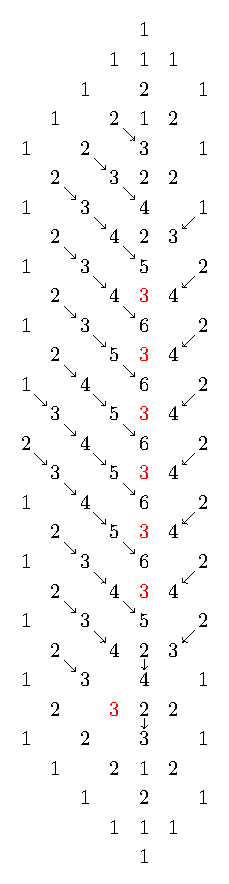
\includegraphics[width=2cm]{figures/E8easy.pdf}
			\subcaption{$E_8$ easy situation}
			}
			\parbox[t]{.2\textwidth}{\centering
			\vspace{0cm}
			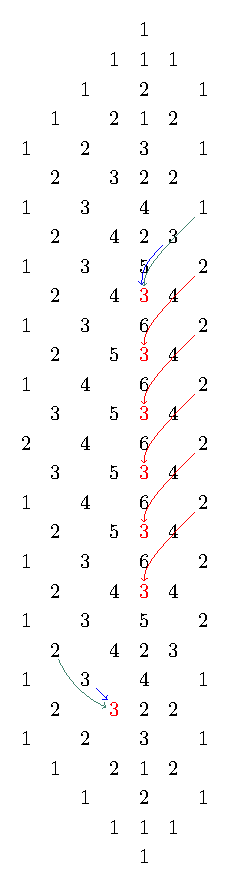
\includegraphics[width=2cm]{figures/E8hard.pdf}
			\subcaption{$E_8$ some exceptions}
			}
			\caption{minimal sectional monos}
			\label{fig:minisecmono}
		\end{figure}
	\end{center}
\begin{remark}
	The condition $\ord(Y)>2$ in the lemma can not be removed.
\end{remark}
\begin{lemma}\label{lem:value}
Let $X \hookrightarrow Y$ be a minimal sectional mono, and $S:=Y/X$ be the quotient. Then we have the short exact sequence 
$$\eta: 0 \longrightarrow X \longrightarrow Y \longrightarrow S \longrightarrow 0$$
and the dimensions of extension groups among $X,Y,S$ are as shown in the Table \ref{table:dim}.
\renewcommand{\arraystretch}{1.1}
%https://tex.stackexchange.com/questions/552563/centering-on-the-last-column-messes-table-up
\begin{table}
\centering
\begin{tabular}{|c|>{ \centering }m{5mm}|>{ \centering }m{5mm}|>{\centering\arraybackslash}m{5mm}|} 
\hline
       \diagbox[height=3.8\line]{$M$}{$[M,N]$\\$[M,N]^1$}{$N$}            & X & Y & S  \\ 
\hline
\multirow{2}{*}{X} & 1 & 1 & 0  \\
                   & 0 & 0 & 0  \\ 
\hline
\multirow{2}{*}{Y} & 0 & 1 & 1  \\
                   & 0 & 0 & 0  \\ 
\hline
\multirow{2}{*}{S} & 0 & 0 & 1  \\
                   & 1 & 0 & 0  \\
\hline
\end{tabular}
\vspace{1mm}
\caption{}
\label{table:dim}
\end{table}

In particular, $S$ is indecomposable and rigid; $[S,X]^1 =1$, so $X_S$ and $S^X$ are well-defined.
\end{lemma}
\begin{proof}
Since every indecomposable representation of Dynkin quiver is a brick, we get $[X,X]=[Y,Y]=1$ and $[X,X]^1=[Y,Y]^1=0$. By the definition of minimal sectional mono, we get
$[X,Y]=1, [Y,X]=0$ and $[X,Y]^1=[Y,X]^1=0$. By applying the functors $[Y,-],[-,S],[X,-],[-,X],[-Y]$ to the short exact sequence $\eta$ we get the results. 
\end{proof}
In the following two lemmas we will describe the representations $S^X$ and $X_S$ more clearly.
\begin{lemma} Take the same notations as in Lemma \ref{lem:value}. Then $S^X=S$.
\end{lemma}
\begin{proof}
	Let $\iota:N \longrightarrow S$ be a proper non-zero subrepresentation of $S$, we need to prove that $\iota^* \eta: 0\longrightarrow X \longrightarrow Y' \longrightarrow N \longrightarrow 0$ splits.
	

\begin{center}
\begin{tikzcd}
\iota^*\eta: & 0 \arrow[r] & X \arrow[r, hook'] \arrow[d, equal] & Y' \arrow[r] \arrow[d, "\eta", hook'] & N \arrow[r] \arrow[d, "\iota", hook'] & 0 \\
\eta:        & 0 \arrow[r] & X \arrow[r]                                       & Y \arrow[r]                           & S \arrow[r]                           & 0
\end{tikzcd}
\end{center}
	
	We decompose $Y'=\oplus_i Y_i'$ as the direct sum of indecomposable representations. Since the map $X\longrightarrow Y$ is the minimal sectional mono, we get $Y_i'=X$ or $Y_i'=Y$ or $X\stackrel{0}{\longrightarrow} Y_i'$ for all $i$.
	If there exists $i$ such that $Y_i'=X$, then $\iota^* $ splits; if there exists $i$ such that $Y_i'=Y$, then $\eta$ is isomorphism, we get $\iota$ is isomorphism; if for every $i$ the map $X \longrightarrow Y_i'$ is $0$, then the map $X \longrightarrow Y'$ is $0$, we also get the contradiction.
\end{proof}

\begin{lemma}[{Follows \cite[Lemma 36]{irelli2019cell}, with the same proof}]\label{lem:descriptionofX_S}
	Let $E \longrightarrow X$ be the minimal right almost split morphism ending in $X$, then we can decompose $E$ as $E=E' \oplus \tau X_1$. When $Y$ is not projective, $X_S$ is isomorphic to $\ker (E \longrightarrow \tau Y) \cong E' \oplus \ker (\tau X_1 \longrightarrow \tau Y)$; when $Y$ is projective, $X_S \cong E$.
\end{lemma}
\begin{corollary}
	When $X \longrightarrow Y$ is irreducible monomorphism, the representation $X_S$ is either $0$ or an indecomposable representation with property that $X_S \longrightarrow X$ is also an irreducible monomorphism.
\end{corollary}
\begin{remark}
	We can not copy everything in \cite[Lemma 56]{irelli2019cell}, sometimes it would happen that $X_S=F \oplus T$ with $F$ and $T$ indecomposable, $F \hookrightarrow X$ is irreducible but $T \longrightarrow X/F$ is not a good mono.
	
	For example, take the quiver of type $E_7$: 
	\[
	\begin{tikzcd}[row sep=3mm, column sep=5mm]
	                &                 &                 & \bullet \arrow[d] &                 &                 \\
	\bullet \arrow[r] & \bullet \arrow[r] & \bullet \arrow[r] & \bullet           & \bullet \arrow[l] & \bullet \arrow[l]
	\end{tikzcd}
	\]
	 take $Y=\representation{122321}{1}$, $X=\representation{112321}{1}$, then $X_S=\representation{111210}{1}\oplus \representation{000111}{0}=F \oplus T$, $X/F =\representation{001111}{0}$, the map $T \longrightarrow X/F$ is not a good mono.
	
	Luckily, we can avoid this bad situation by carefully choosing the minimal sectional mono $X \longrightarrow Y$. The minimal sectional monos I chose are presented in Figure \ref{fig:minisecmono}. In appendix we will write down the induction process in detail for some examples.
\end{remark}

Now we analyse every case in Figure \ref{fig:minisecmono}, i.e., prove Claim \ref{claim:bigorder} by cases. For convenience we omit subscripts which indicate the dimension vectors. 

\begin{proof}[{Proof of Claim \ref{claim:bigorder}}]
When the minimal sectional mono $X \longrightarrow Y$ is irreducible, we use Theorem \ref{thm:main2} to get morphism
$$\Grr(\Phi(Y)) \longrightarrow \Grr(\Phi(X)) \shorttimes \Grr(\Phi(S)) \oder \Grr(\Phi(X)) \setminus \Grr(\Phi(X_S)).$$ 
By observation of  Figure \ref{fig:minisecmono}, $\orde(S)=\orde(Y)-\orde(X)$ is smaller or equal to $2$, so by Lemma \ref{lem:smallvecdim} $\Gr(\Phi(S))$ has the affine paving property. Let $Y_1:=X$, $X_1:=X_S$, $S_1:=Y_1/X_1$, we again use Theorem \ref{thm:main2} to get Zariski-locally affine maps
\begin{equation*}
\begin{aligned}
\Grr(\Phi(X)) &\longrightarrow \Grr(\Phi(X_1)) \shorttimes \Grr(\Phi(S_1)) \oder \Grr(\Phi(X_1)) \setminus \Grr(\Phi(X_{1S_1}))\\
\Grr(\Phi(X))\setminus \Grr(\Phi(X_S))&\longrightarrow \Grr(\Phi(X_1)) \shorttimes \Grr(\Phi(S_1)).
\end{aligned}
\end{equation*}
Luckily $\orde(S_1)$ is still smaller or equal to $2$. We can continue this process until the order of representations are small enough.

The exceptional cases are similar, but the discussion is a bit more complicated. Let us look at some examples. (We simplify the notations: $\Gr(M)$ as $\Grr_{\dimvec{f}}(\Phi(M))$, $U(M,N)$ as $\Grr_{\dimvec{f}}(\Phi(M)) \setminus \Grr_{\dimvec{f}}(\Phi(N))$, and we also ignore the dimension vectors.)
\captionsetup[subfigure]{labelfont=rm}
\captionsetup[subfigure]{labelformat=parens}
%https://tex.stackexchange.com/questions/233481/subcaption-defaulting-to-capital-letter-labels
	\begin{center}
		\begin{figure}[ht]
			\vspace{0cm}
			\parbox[b]{.23\textwidth}{\centering
			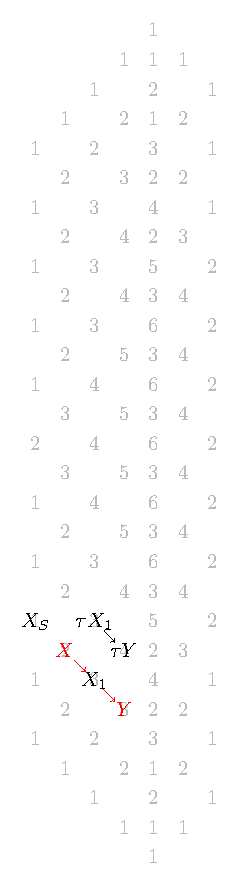
\includegraphics[width=3.2cm]{figures/E8graypic1.pdf}
			\subcaption{}
			}
			\parbox[b]{.23\textwidth}{\centering
			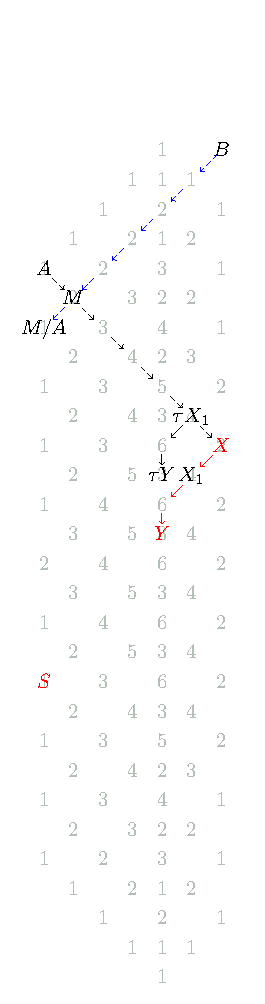
\includegraphics[width=3.2cm]{figures/E8graypic2.pdf}
			\subcaption{}
			}
			\parbox[b]{.23\textwidth}{\centering
			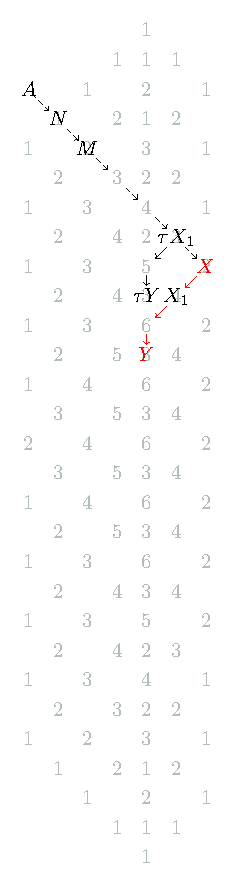
\includegraphics[width=3.2cm]{figures/E8graypic3.pdf}
			\subcaption{}
			}
			\parbox[b]{.23\textwidth}{\centering
			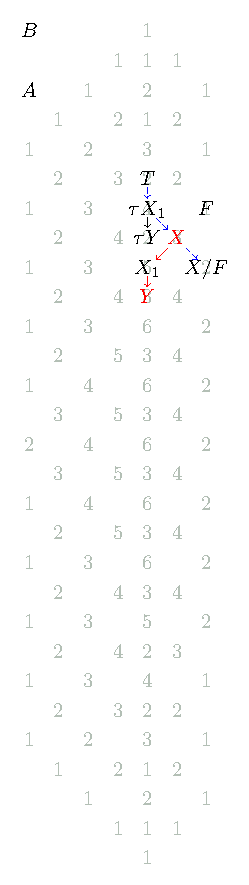
\includegraphics[width=3.2cm]{figures/E8graypic4.pdf}
			\subcaption{}
			}
			\caption{special cases}
			\label{fig:specialcases}
			\vspace{0.2cm}
		\end{figure}
	\end{center}
\begin{eg}
In the case of Figure \ref{fig:specialcases}(a), if $X_1 \longrightarrow Y$ is injective, then we obtain some Zariski-locally affine maps
\begin{equation*}
\begin{aligned}
\Gr(Y) &\longrightarrow \Gr(X_1) \shorttimes \Gr(Y/X_1) \oder U(X_1,X)\\
\Gr(X_1) &\longrightarrow \Gr(X) \shorttimes \Gr(X_1/X) \oder U(X,X_S)\\
U(X_1,X) &\longrightarrow \Gr(X) \shorttimes \Gr(X_1/X) \\
U(X,X_S) &\longrightarrow \Gr(X_S) \shorttimes \Gr(X/X_S). \\
\end{aligned}
\end{equation*}

When $X_1 \longrightarrow Y$ is not injective, we get
$$\Gr(Y) \longrightarrow \Gr(X) \shorttimes \Gr(Y/X) \oder U(X,X_S).$$
Since the map $\tau X_1 \longrightarrow \tau Y$ is injective, from Lemma \ref{lem:descriptionofX_S} we get $X_S\longrightarrow X$ is irreducible monomorphism. Thus
$$U(X,X_S) \longrightarrow \Gr(X_S) \shorttimes \Gr(X/X_S).$$
These maps give the variety $\Gr(Y)$ an affine paving from bottom to top.
\end{eg}
\begin{eg}
In Figure \ref{fig:specialcases}(b), we would like to prove that  $\Gr(Y)$ has the affine paving property. We have
$$\Gr(Y) \longrightarrow \Gr(X) \shorttimes \Gr(Y/X) \oder U(X,X_S).$$
When the map $M \longrightarrow X$ is not monomorphism, we get
$$U(X,X_S) \longrightarrow \Gr(X_S) \shorttimes \Gr(X/X_S);$$
when the map $M \longrightarrow X$ is monomorphism, we get
\begin{equation*}
\begin{aligned}
U(X,X_S)&=U(X,M) \bigsqcup U(M,X_S)\\
U(X,M) &\longrightarrow \Gr(M) \shorttimes \Gr(X/M)\\
U(M,X_S) &\longrightarrow \Gr(X_S) \shorttimes \Gr(M/X_S).
\end{aligned}
\end{equation*}
Since the order of $X$, $Y/X$, $X_S$, $X/X_S$, $M$, $X/M$, $M/X_S$ are smaller or equal to $2$, the induction process stops, we get $\Gr(Y)$ has the affine paving property.
\end{eg}
\begin{eg}
In the case of Figure \ref{fig:specialcases}(c), we have 
$$\Gr(Y) \longrightarrow \Gr(X) \shorttimes \Gr(Y/X) \oder U(X,X_S)$$
where $X_S=\ker(\tau X_1 \longrightarrow \tau Y)$. When $X_S=0$ we're done; if not, then $A \neq 0$ and $X_S=A$, we decompose $X_S \longrightarrow Y$ as compositions of minimal sectional monos:

Case 1: $M\longrightarrow X$ is not injective, then
 \begin{equation*}
 \begin{aligned}
 U(X,X_S)&=U(X,N) \bigsqcup U(N,X_S)\\
 U(X,N) &\longrightarrow \Gr(N) \shorttimes \Gr(X/N)\\
 U(N,X_S) &\longrightarrow \Gr(X_S) \shorttimes \Gr(N/X_S).
 \end{aligned}
 \end{equation*}
 
 Case 2: $M\longrightarrow X$ is injective, then
  \begin{equation*}
  \begin{aligned}
  U(X,X_S)&=U(X,M) \bigsqcup U(M,N) \bigsqcup U(N,X_S)\\
  U(X,M) &\longrightarrow \Gr(M) \shorttimes \Gr(X/M)\\
  U(M,N) &\longrightarrow \Gr(N) \shorttimes \Gr(M/N)\\
  U(N,X_S) &\longrightarrow \Gr(X_S) \shorttimes \Gr(N/X_S).
  \end{aligned}
  \end{equation*}
  
  Since $\Gr(X)$, $\Gr(Y/X)$, $\Gr(N)$, $\ldots$ have affine paving property, we conclude that $\Gr(Y)$ has also the affine paving property.
\end{eg}
\begin{eg}
Finally we begin to tackle the most difficult case(Figure \ref{fig:specialcases}(d)). When $X \longrightarrow Y$ is not injective, we get
$$\Gr(Y) \longrightarrow \Gr(F) \shorttimes \Gr(Y/F) \oder U(F,?),$$
and then we get the result.\footnote{$\Gr(F)$ is empty or a singleton, so is $U(F,?)$, no matter what representation is in the questionmark.}

When $X \longrightarrow Y$ is injective, we have
$$\Gr(Y) \longrightarrow \Gr(X) \shorttimes \Gr(Y/X) \oder U(X,X_S)$$
where $X_S=F\oplus \ker(\tau X_1 \longrightarrow \tau Y)=F \oplus T$ by Lemma \ref{lem:descriptionofX_S}. Since $X \longrightarrow Y$ is injective, we get $A=0$, thus $B=0$ also, and then the sectional map $T \longrightarrow X/F$ in injective. We thus get two short exact sequence satisfying the conditions in \ref{thm:main2}:
\begin{center}
% https://tikzcd.yichuanshen.de/#N4Igdg9gJgpgziAXAbVABwnAlgFyxMJZARgBoAGAXVJADcBDAGwFcYkRyQBfU9TXfIRQAmCtTpNW7AGLdeIDNjwEiAZjE0GLNohAANOXyWCiAFg0Tt7PQHpZPIwJUoArBa1TdnBwv7KhJKTE4h46HIa+xs7IbsGakmHe8opOAaJxlp4gACoRKf5qQSEJ1nZ5fiYo5hmhpXoA+gDK5VEB5O4lugA6XTA49Lo++ZXI7TWdID0AHliD4jBQAObwRKAAZgBOEAC2SG4gOBBIAOw+mzsnNIdIABxnW7uIN1dHiACc8VbdXWhYAOQRc6PD4HV4ANnuF0Q6lBSFMkMeolh0M+WR6v0BDyQZGRwgRSHayOIXEoXCAA
\begin{tikzcd}[row sep=0mm]
\eta: & 0 \arrow[r] & F \arrow[r] & X \arrow[r, "\pi"]    & X/F \arrow[r]   & 0 \\
\xi:  & 0 \arrow[r] & T \arrow[r] & X/F \arrow[r, "\pi'"] & X/X_S \arrow[r] & 0.
\end{tikzcd}
\end{center}
Let $N \in \Gr(X)$ be a subrepresentation, it is obvious that $N \in \Gr(X_S) \iff \pi'\circ \pi(N)=0$, so 
  \begin{equation*}
  \begin{aligned}
  N\in U(X,X_S) & \iff \pi'\circ \pi(N) \neq 0\\
  & \iff \pi(N) \notin \Gr(T)\\
  & \iff \pi(N) \in U(X/F,T)\\
  & \iff \Psi_{\eta}(N) \in \Gr(F) \times U(X/F,T).
  \end{aligned}
  \end{equation*}
\end{eg}
Thus the Zarisky-locally trivial affine bundle map
$$U(X,F) \longrightarrow \Gr(F) \shorttimes \Gr(X/F)$$
restricted to the Zarisky-locally trivial affine bundle map
$$U(X,X_S) \longrightarrow \Gr(F) \times U(X/F,T).$$

Finally, by applying the short exact sequence $\xi$ to Theorem \ref{thm:main2}, we get the map
$$U(X/F,T) \longrightarrow \Gr(X/F) \shorttimes \Gr(T).$$
Since all the Grassmannians $\Gr(X)$, $\Gr(Y/X)$, $\Gr(F)$, $\Gr(X/F)$, $\Gr(T)$ have the affine paving property, we conclude that $\Gr(Y)$ has the affine paving property.
\end{proof}
\bibliographystyle{plain}
\bibliography{reference}





\end{document}




